%\documentclass[a4paper]{article}
\documentclass[11pt]{extarticle}

\usepackage[utf8]{inputenc}
\usepackage{listings}
\usepackage{lipsum}
\usepackage{hyperref}
\usepackage{amssymb}
\usepackage[english]{babel}
\usepackage[numbered,framed]{matlab-prettifier}
\usepackage[useregional]{datetime2}
\usepackage{graphicx}

\lstset{
  style              = Matlab-editor,
  basicstyle         = \mlttfamily,
  escapechar         = ",
  mlshowsectionrules = true,
}

\title{\vspace{2cm}Elaborato di\\ \textbf{Calcolo Numerico}\\ Anno Accademico 2016/2017\vspace{1cm}}

\author{Gabriele Puliti - \texttt{5300140} - \href{mailto:gabriele.puliti@stud.unifi.it}{\textit{gabriele.puliti@stud.unifi.it}}
\and Luca Passaretta - \texttt{ } - \href{mailto: }{\textit{ }}}

\date{}

\addto\captionsenglish{\renewcommand{\contentsname}{Capitoli}}

\begin{document}

\maketitle

\begin{center}
\today{}
\end{center}

\newpage
\
\newpage

\tableofcontents
\newpage
\
\newpage

\section{\textbf{Capitolo 1}}
\subsection{Esercizio 1}
Sapendo che il metodo iterativo è convergente a \( x^* \) allora per definizione si ha:
 \[
	\lim_{k \to +\infty}\ x_k = x^*
\]
 inoltre per definizione di \( \Phi \) si calcola il limite:
\[
    \lim_{k \to +\infty} \Phi(x_k) = \lim_{k \to +\infty} x_{k+1} = x^*
\]
 infine ipotizzando che la funzione \( \Phi \) sia uniformemente continua, è possibile calcolare il limite:
\[
    \lim_{k \to +\infty} \Phi(x_k) = \Phi(\lim_{k \to +\infty} x_k) = \Phi(x^*)
\]
 dai due limiti si ha la tesi:
\[
    \Phi(x^*) = x^* 
\]
\subsection{Esercizio 2}
Dal momento che le variabili intere di 2 byte in Fortran vengono gestite in Modulo e Segno, la variabile \texttt{n}, inizializzata con

\begin{lstlisting}
integer*2 n
\end{lstlisting}
varia tra \( - 2^{15} \leq n \leq 2^{15} - 1 \) e quindi tra  \( -32768 \leq n \leq 32767 \). \\
Andando quindi ad eseguire la somma \( (32767+1)_{10} = (0111111111111111 + 1)_{2,MS} = \\
= (11111111111111111)_{2,MS} = (-327628)_{10} \)

\subsection{Esercizio 3}
Per definizione si ha che la precisione di macchina \(u\), per arrotondamento e' data da:
\[
u=\frac{1}{2} b ^{1-m}
\]
Se \(b=8, m=5\) si ha:
\[ 
u = \frac{1}{2}\cdot 8^{1-5} = \frac{1}{2}\cdot 8^{-4} = 1,2 \cdot 10^{-4} 
\]

\newpage
\subsection{Esercizio 4}
Il codice seguente:
\lstinputlisting[language=Matlab]{cap_1/es4/es4.m}
restituisce questo risultato (assumendo che $f(x)$ = $ e^x $ e $ x_0 = 0 $ ): 
\begin{center}
\begin{tabular}{c|c}
h & \( \Psi_{h}(0) \)  \\
\hline
    \(10^{-1}\) & 1.051709180756477e+00\\
    \(10^{-2}\) & 1.005016708416795e+00\\
    \(10^{-3}\) & 1.000500166708385e+00\\
    \(10^{-4}\) & 1.000050001667141e+00\\
    \(10^{-5}\) & 1.000005000006965e+00\\
    \(10^{-6}\) & 1.000000499962184e+00\\
    \(10^{-7}\) & 1.000000049433680e+00\\
    \(10^{-8}\) & 9.999999939225290e-01\\
    \(10^{-9}\) & 1.000000082740371e+00\\
    \(10^{-10}\) & 1.000000082740371e+00\\
    \(10^{-11}\) & 1.000000082740371e+00\\
    \(10^{-12}\) & 1.000088900582341e+00\\
\end{tabular} \\
\end{center}
si può notare che al diminuire del valore h, la funzione \(\Psi_{h}(0)\) approssima con maggior precisione il valore $f'(0)$, come si può vedere dal plot \ref{fes14}.
\subsection{Esercizio 5}
Tesi:\\
Sia f(x) una funzione sufficentemente regolare e h>0 una quantità ``piccola''\\
Ipotesi:\\
\[
\frac{f(x_0 + h) - f(x_0 + h)}{2h} = f'(x_0) + O(h^2)
\]
\[
\frac{f(x_0 + h) -2f(x_0) - f(x_0 + h)}{h^2} = f''(x_0) + O(h^2)
\]

Dimostrazione:\\
Sviluppiamo la funzione f(x) mediante il polinomio di taylor al secondo ordine\\
\[
f(x) = f(x_0) + (x-x_0)f'(x_0)+\frac{(x-x_0)^2}{2}f''(x_0) + O((x-x_0)^3)
\]
Sostituiamo \[x=(x_0 +h)\] e  \[x=(x_0-h)\]
\[
f((x_0 +h) = f(x_0) + hf'(x_0)+\frac{h^2}{2}f''(x_0) + O(h^3)
\]
\[
f((x_0 -h) = f(x_0) - hf'(x_0)+\frac{h^2}{2}f''(x_0) + O(h^3)
\]
Risostituendo  nel rapporto incrementale dell'ipotesi otteniamo:
\[
\frac{ f(x_0) + hf'(x_0)+\frac{h^2}{2}f''(x_0) + O(h^3) - f(x_0) - hf'(x_0)+\frac{h^2}{2}f''(x_0) + O(h^3)}{2h} = \frac{2hf'(x_0) + O(h^3)}{2h} =f'(x_0) + O(h^2)
\]

Per la seconda uguaglianza dell'ipotesi basterà applicare lo stesso procedimento con uno sviluppo di taylor al 3° ordine.
\subsection{Esercizio 6}
Il codice MatLab, indicando con x=$x_n$ e r=$\epsilon$:
\lstinputlisting[language=Matlab]{cap_1/es6/es6.m}
\newpage
restituisce i valori:
\begin{center}
\begin{tabular}{c|c|c}
n & $x_n$ & $\epsilon$ \\
\hline
    0 & 2.00000000000000e+000 & 585.786437626905e-003\\
    1 & 1.50000000000000e+000 & 85.7864376269049e-003\\
    2 & 1.42857142857143e+000 & 14.3578661983335e-003\\
    3 & 1.41463414634146e+000 & 420.583968367971e-006\\
    4 & 1.41421568627451e+000 & 2.12390141496321e-006\\
    5 & 1.41421356268887e+000 & 315.774073555986e-012\\
    6 & 1.41421356237310e+000 & 0.00000000000000e+000\\
    7 & 1.41421356237310e+000 & 0.00000000000000e+000\\
\end{tabular}
\end{center}
I valori indicano che per valori di $n$ superiori a 5 l'errore, indicato con $\epsilon$, è dell'ordine di \(10^{-12}\).
\subsection{Esercizio 7}
Sapendo che la rappresentazione del numero è stata fatta usando l'arrotondamento, la precisione di macchina si calcola:
\[
u = \frac{b^{1-m}}{2}
\]
il cui valore sappiamo essere pari a:
\[
u \approx 4.66 \cdot 10^{-10}
\]
dato che stiamo cercando il numero di cifre binarie allora si deve avere $b=2$, è quindi possibile ricavare $m$:
\[
m = 1- log_2{(4.66 \cdot 10 ^{-10})} \approx 31.99
\]
possiamo pertanto affermare che servono 32 cifre dedicate alla mantissa per rappresentare il numero con precisione macchina \(4.66 \cdot 10^{-10}\).
\subsection{Esercizio 8}
Sapendo che la mantissa in decimale è calcolabile tramite la funzione:
\begin{itemize}
\item \( m = 1- log_{10}{u} \) (troncamento) 
\item \( m = 1- log_{10}{(2\cdot u)} \) (arrotondamento)
\end{itemize}
e che la precisione di macchina assuma un valore accettabilemente piccolo in modo tale che il \(log_{10}{u} \approx 1\), cioè $0<=u<1$, allora è possibile scrivere:
\begin{itemize}
\item \( m = 1 - log_{10}{u} \approx -log_{10}{u} \) (troncamento)
\item \( m = 1 - log_{10}{2u} = 1 - log_{10}{2} - log_{10}{u} \approx -log_{10}{u} \) (arrotondamento)
\end{itemize}
\subsection{Esercizio 9}
\lstinputlisting[language=Matlab]{cap_1/es9/es9.m}
Il valore di delta è uguale a \(\frac{1}{10}\), la rappresentazione binaria di questo numero però non è esatta.
Si tratta di una rappresentazione periodica e quindi, in decimale, sarà circa 0.0999, prendendo quindi $delta\approx0.9$ vedremo che per $i=10$ $x\approx0.999$, mentre per $i=11$  $x\approx1,0989$. Per questo motivo la condizione x=1 non si avvererà mai e il programma non terminerà.
\subsection{Esercizio 10}
Il calcolo della radice e dell'elevamento a potenza è sempre ben condizionato.  La parte problematica è l'overflow della somma.
Troviamo quindi il massimo dei due addendi:\\
\begin{equation}
m = max\{|x|,|y|\} 
\end{equation}
\begin{equation}
\sqrt{x^2 + y^2}
\end{equation}
Dividiamo entrambi i membri per il massimo
\begin{equation}
\sqrt{m^2*(\frac{x}{m}^2 + \frac{y}{m}^2)}
\end{equation}
Portiamo fuori il massimo dalla radice
\begin{equation}
m*\sqrt{\frac{x}{m}^2 + \frac{y}{m}^2}
\end{equation}

\subsection{Esercizio 11}
L'espressione aritmetica dei due algoritmi è:\\
\begin{itemize}
\item{1)} (x+y)+z = x+y+z 
\item{2)}  x+(y+z) = x+y+z 
\end{itemize}
Ne consegue che sono equivalenti
In aritmetica finita, invece, avremo:
\begin{itemize}
\item{1)} \( (x\oplus y)\oplus z = fl(fl(fl(x) + fl(y)) +fl(z)) = \)\\
\( =((x(1+\varepsilon_x) + y(1+\varepsilon_y))(1+\varepsilon_A) +z(1+\varepsilon_z))(1+\varepsilon_B) = \) \\
\[\varepsilon_R =\frac{(x(1+\varepsilon_x)(1+\varepsilon_A)(1+\varepsilon_B) + y(1+\varepsilon_y)(1+\varepsilon_A)(1+\varepsilon_B)+z(1+\varepsilon_z))(1+\varepsilon_B) -x-y-z}{z+y+z}     \]
prendo \( \varepsilon_M = max\{\varepsilon_x, \varepsilon_y, \varepsilon_z, \varepsilon_A, \varepsilon_B\}\)
\[\varepsilon_R \leq \frac{x(1+\varepsilon_M)^3 + y(1+\varepsilon_M)^3+z(1+\varepsilon_M)^2 -x-y-z}{z+y+z} = \]
\[ =  \frac{x(3\varepsilon_M + 3\varepsilon_M^2 +\varepsilon_M^3) + y(3\varepsilon_M + 3\varepsilon_M^2 +\varepsilon_M^3)+z(2\varepsilon_M + \varepsilon_M^2)}{z+y+z}    \]
Sapendo che \(\varepsilon_M \leq 1 \) posso affermare che \( \varepsilon_M \geq \varepsilon_M^2 \geq \varepsilon_M?3 \) ed effettuare un'altra minorazione

\[ \varepsilon_R \leq \frac{7x\varepsilon_M + 7y\varepsilon_M + 3z\varepsilon_M}{x+y+z} = \varepsilon_M(3+4\frac{x+y}{x+y+z}) \]

\item{2)}  \( x\oplus (y\oplus z) =fl(fl(x) +fl( fl(y) +fl(z)))     \) \\
Il procedimento sarà analogo a quello visto prima con lo scambio degli addendi al nominatore della frazione
\[ \varepsilon_R \leq \frac{7z\varepsilon_M + 7y\varepsilon_M + 3x\varepsilon_M}{x+y+z} = \varepsilon_M(3+4\frac{z+y}{x+y+z}) \]
\end{itemize}
\subsection{Esercizio 12}
Ipotesi: k sia il numero di condizionamento di:
\[
y = \sqrt{x}
\]
Tesi:
\[
k=\frac{1}{2}
\]
\[
f(x) = \sqrt{x}
\]
\[
f'(x) = \frac{1}{2\sqrt{x}}
\]
\[
k \equiv |f'(x) \cdot \frac{x}{y} | = | \frac{1}{2\sqrt{x}} \cdot \frac{x}{ \sqrt{x} } | = | \frac{1}{2} \cdot \frac{x}{x} | = | \frac{1}{2}|
\]
\[ \blacksquare \]

\subsection{Esercizio 13}
Il problema è che stiamo rappresentando dei numeri reali in un calcolatore quindi la loro rappresentazione comporta delle approssimazioni. Nella riga 11 abbiamo calcolato e restituito in output il valore interno al logaritmo $\big|3(1-\frac{3}{4})+1\big|$ che teoricamente è zero, ma si ottiene $ 2.220446049250313e-16 $. 
Si può vedere che il codice MatLab:
\lstinputlisting{cap_1/es13/es13.m}
calcola i valori della funzione ottenendo il grafico \ref{fes113} e si può notare che l'asintoto verticale in $x=\frac{4}{3}$ viene rappresentato come minimo della funzione $f(x)$.

\section{\textbf{Capitolo 2}}
\underline{Le funzioni usate nei codici seguenti sono in fondo al capitolo} (pag. \pageref{functcap2})
\subsection{Esercizio 1}
Per ricercare la radice quadrata di un numero è possibile sfruttare una modifica al problema delle radici di una funzione. Infatti partendo da $x=\sqrt{\alpha}$ è possibile svilupparla trovando una funzione $f(x)$ utilizzabile nel metodo di Newton:
\[
x = \sqrt{\alpha} 
\]
\[
x^{2} = \big(\sqrt{\alpha}\big)^{2} 
\]
\[
x^{2} - \alpha = 0
\]
possiamo quindi considerare $f(x) = x^{2} - \alpha$ e $f'(x) = 2\cdot x$ . La procedura iterativa è definita quindi da:
\[
x_{n+1} = x_{n} - \frac{f(x_{n})}{f'(x_{n})} = x_{n}-\frac{x_{n}^2-\alpha}{2\cdot x_{n}} = x_{n} - \frac{x_{n}}{2} + \frac{\alpha}{2\cdot x_{n}} = \frac{x_{n}}{2}+\frac{\alpha}{2\cdot x_{n}} = \frac{1}{2} \cdot \Big(x_{n}+\frac{\alpha}{x_{n}}\Big)
\]
che ci permette di implementare il seguente script matlab e la funzione y = NewtonSqrt(alpha, x\_0, imax, tol):
\lstinputlisting[language=matlab]{cap_2/es1/es1.m}
Che restituisce in output valori che abbiamo rappresentato nella tabella seguente:
\begin{center}
\begin{tabular}{|c|c|}
\hline
$i$ & \( x_i \) \\
\hline
1 & 1.750000000000000e+00 \\
2 & 1.732142857142857e+00 \\
3 & 1.732050810014727e+00 \\
4 & 1.732050807568877e+00 \\
\hline
\end{tabular}\\
\end{center}
\subsection{Esercizio 2}
\begin{flushleft}
E' possibile effettuare gli stessi passaggi dell'esercizio precedente, ricordandosi che la radice in questo caso non è quadrata ma ennesima:
\[
x = \sqrt[n]{\alpha} 
\]
\[
x^{n} = \big(\sqrt[n]{\alpha}\big)^{n} 
\]
\[
x^{n} - \alpha = 0
\]
consideriamo quindi la funzione $f(x) = x^{n} - \alpha$ e $f'(x) = n\cdot x^{n-1}$ . La procedura iterativa è definita quindi da:
\[
x_{n+1} = x_{n} - \frac{f(x_{n})}{f'(x_{n})} = x_{n}-\frac{x_{n}^n-\alpha}{n\cdot x_{n}^{n-1}} = x_{n} - \frac{x_{n}}{n} + \frac{\alpha}{n\cdot x_{n}^{n-1}} = 
\]
\[
= \Big((n-1)\cdot x_n- \frac{\alpha}{x_n^{n-1}}\Big) \cdot \frac{1}{n} = \frac{\Big( (n-1)\cdot x_n^{n}+\alpha\Big)}{n\cdot x_n^{n-1}}
\]
La radice da approssimare in questo caso ha grado ennesimo quindi sono necessarie delle modifiche alla funzione matlab usata nell'esercizio precedente che chiamiamo y = NewtonSqrt(n, alpha, x\_0, imax, tol). Lo script MatLab corrispondente ai casi $n = 3,4,5$ è il seguente:
\lstinputlisting[language=Matlab]{cap_2/es2/es2.m}
Mostriamo l'output in forma tabellare con $i$ che rappresenta le iterazioni del metodo e $x_i$ i relativi risultati:
\begin{center}
\begin{tabular}{|c|c|c|c|}
\hline
i & $x_i$ con $n=3$ & $x_i$ con $n=4$ & $x_i$ con $n=5$\\
\hline
1 & 1.631784138709347e+00 & 1.771797299323380e+00 & 1.943788863498140e+00 \\
2 & 1.463411989089094e+00 & 1.463688102853308e+00 & 1.597060655491283e+00 \\
3 & 1.442554125137959e+00 & 1.336940995805593e+00 & 1.369877122538772e+00 \\
4 & 1.442249634601091e+00 & 1.316557487370408e+00 & 1.266284124539191e+00 \\
5 & 1.442249570307411e+00 & 1.316074279204018e+00 & 1.246387399421677e+00 \\
6 & ------------ & 1.316074012952573e+00 & 1.245731630753065e+00 \\
7 & ------------ & ------------ & 1.245730939616284e+00 \\
\hline
\end{tabular}
\end{center}
\end{flushleft}
\subsection{Esercizio 3}
Per confrontare il metodo delle secanti con quello di Newton abbiamo creato il codice MatLab:
\lstinputlisting[language=matlab]{cap_2/es3/es3.m}
I risultati ottenuti dall'utilizzo del metodo delle secanti sono: \newline
\\
\scalebox{0.9} {
\begin{tabular}{c|c|c|c|c}
i & metodo di Newton & metodo delle secanti & \big|newton-$\sqrt{2}$\big| & \big|secanti-$\sqrt{2}$\big|\\
\hline
1 & 1.750000000000000e+00 & 1.736842105263158e+00 & 3.357864376269049e-01 & 3.226285428900628e-01 \\
2 & 1.732142857142857e+00 & 1.732142857142857e+00 & 3.179292947697618e-01 & 3.179292947697618e-01 \\
3 & 1.732050810014727e+00 & 1.732050934706042e+00 & 3.178372476416318e-01 & 3.178373723329468e-01 \\
4 & --------- & 1.732050807572255e+00 & ------- & 3.178372451991598e-01\\
\end{tabular}
}
\\ \newline
Si nota dalla tabella che \( \big|newton-\sqrt{2}\big| \approx  \big|secanti-\sqrt{2}\big| \), cioè che l'ordine di grandezza dell'errore assoluto tra i due metodi è lo stesso. Si può quindi affermare che l'uso del metodo di Newton o del metodo delle secanti è equivalente.
\newpage
\subsection{Esercizio 4}
\begin{flushleft}
Abbiamo scritto delle funzioni MalLab che ci permettono di effettuare il raffronto tra i vari metodi (in ordine: metodo di Newton, metodo di Newton modificato, metodo di accelerazione di Aitken), è possibile vederle a pag. \pageref{functcap2}. Scritte le Function, le abbiamo usate nel seguente script: 
\lstinputlisting[language=Matlab]{cap_2/es4/es4.m}
Questo codice esegue i metodi di Newton, Newton modificato e Aitken per le funzioni date. Rispetto alla funzione $f_1(x)=(x-\pi)^{10}$ rappresentiamo l'output del codice precedente in forma tabellare: 
\begin{center}
\begin{tabular}{|c|c|c|c|}
\hline
tolx & Newton & Newton modificato & Aitken \\
\hline
$10^{0}$ & 4.814159265358979 & 4.814159265358979 & 2.666666666666667 \\
$10^{-1}$ & 4.030463126315021 & 4.030463126315021 & 3.141592653589783 \\
$10^{-2}$ & 3.229126031324792 & 3.229126031324792 & 3.141592653589783 \\
$10^{-3}$ & 3.150212685926121 &  3.150212685926121 &  3.141592653589783 \\ 
$10^{-4}$ & 3.150212685926121 & 3.150212685926121 & 3.141592653589783 \\
$10^{-5}$ & 3.150212685926121 & 3.150212685926121 & 3.141592653589783 \\
\hline
\end{tabular}
\end{center}
Rispetto alla funzione $f_2(x) = (x-\pi)^{10} \cdot e^{2\cdot x}$ si hanno invece i valori:
\begin{center}
\begin{tabular}{|c|c|c|c|}
\hline
tolx & Newton & Newton modificato & Aitken \\
\hline
$10^{0}$ & 4.864516114854061 & 4.864516114854061 & 3.068982105941251 \\
$10^{-1}$ & 4.200823975656096 & 4.200823975656096 & 3.140645194956157 \\
$10^{-2}$ & 3.226469748549500 & 3.226469748549500 & 3.141592492095279 \\
$10^{-3}$ & 3.154537411727535 & 3.154537411727535 &  3.141592492095279 \\ 
$10^{-4}$ & 3.154537411727535 & 3.154537411727535 & 3.141592516390607 \\
$10^{-5}$ & 3.154537411727535 & 3.154537411727535 & 3.141592516390607 \\
\hline
\end{tabular}
\end{center}
Abbiamo poi riportato il plot matlab relativo ai precedenti valori:
\begin{figure}[H]
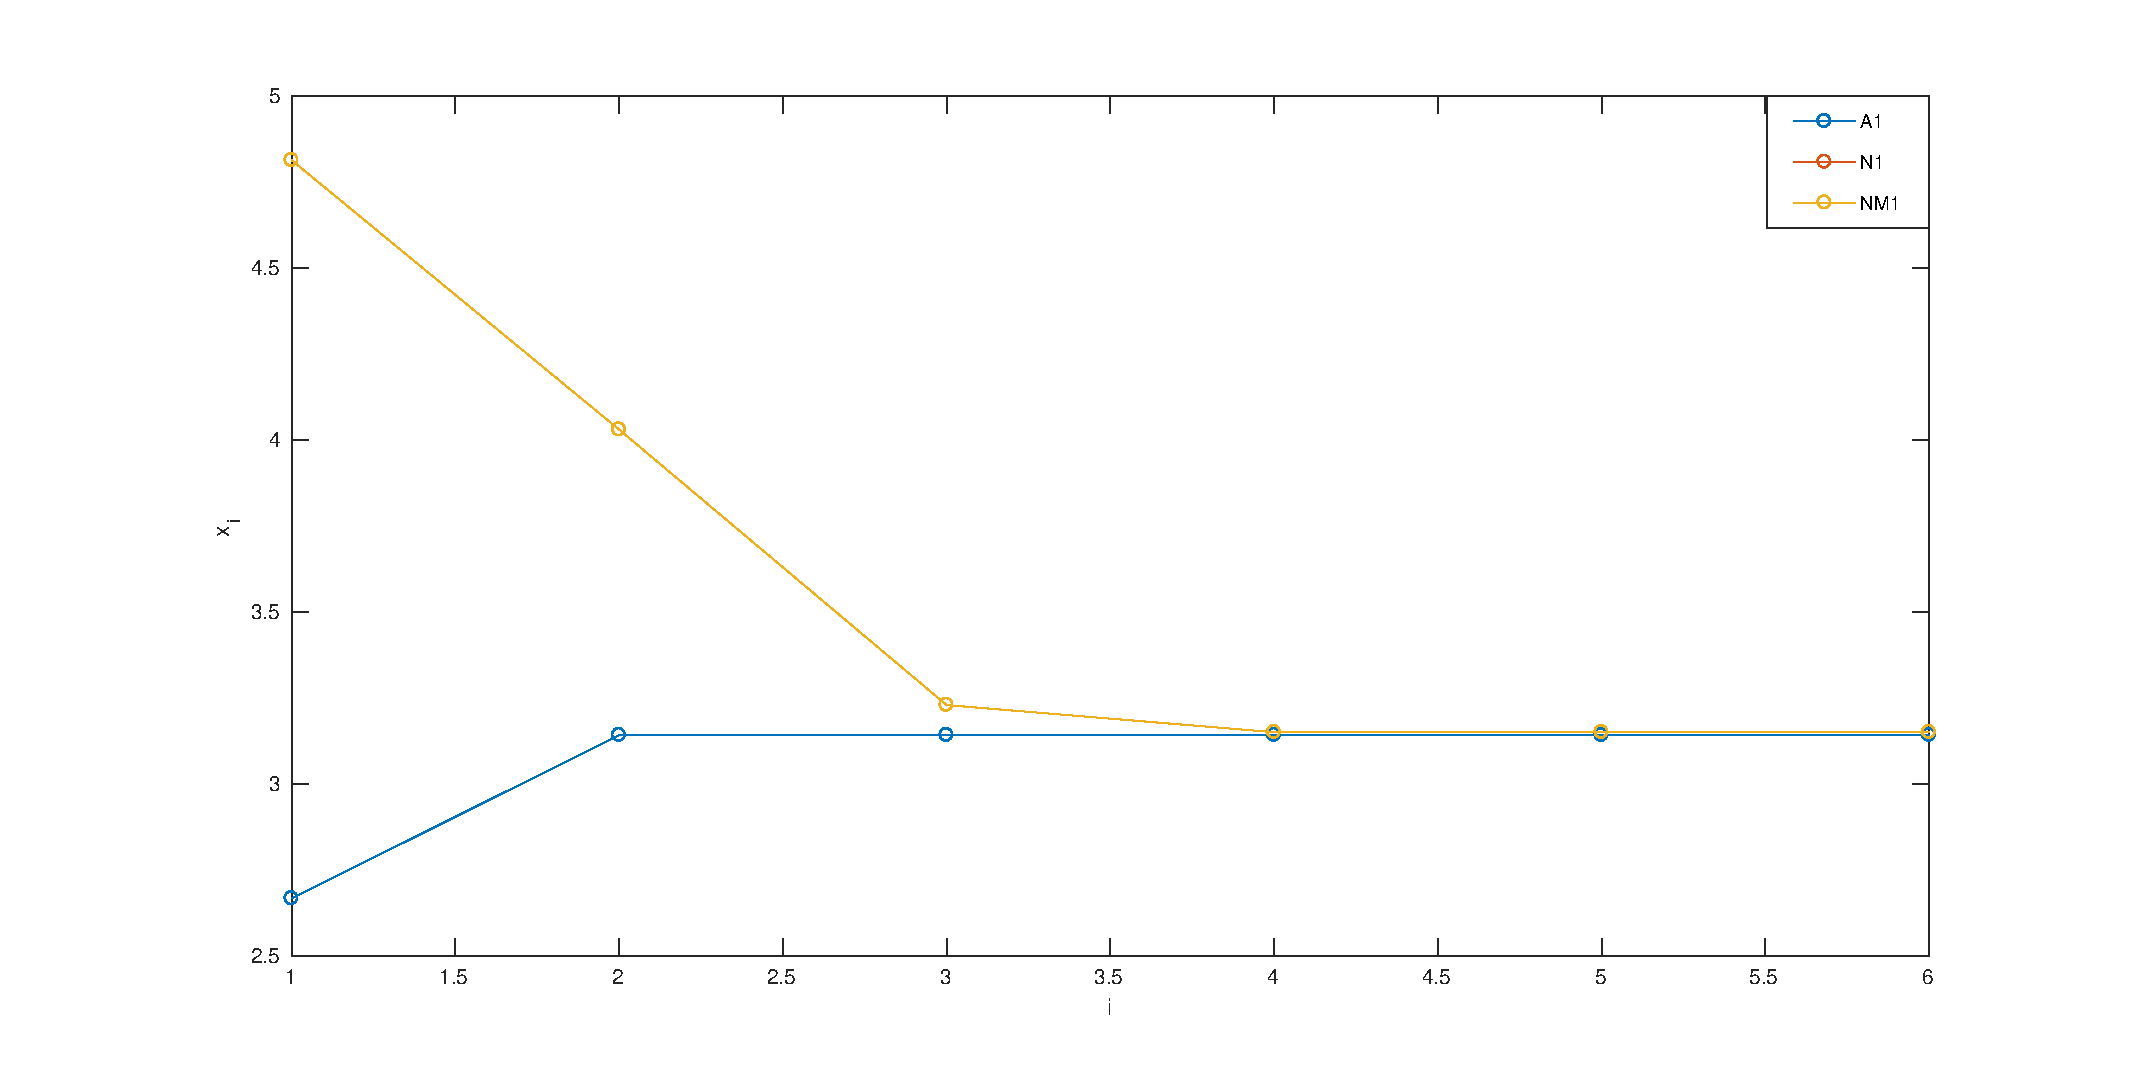
\includegraphics[left, width=210px]{plot/fes24a.eps}
\caption{Andamento del calcolo degli zeri della funzione $f_1(x)=(x-\pi)^{10}$ al variare della tolleranza}
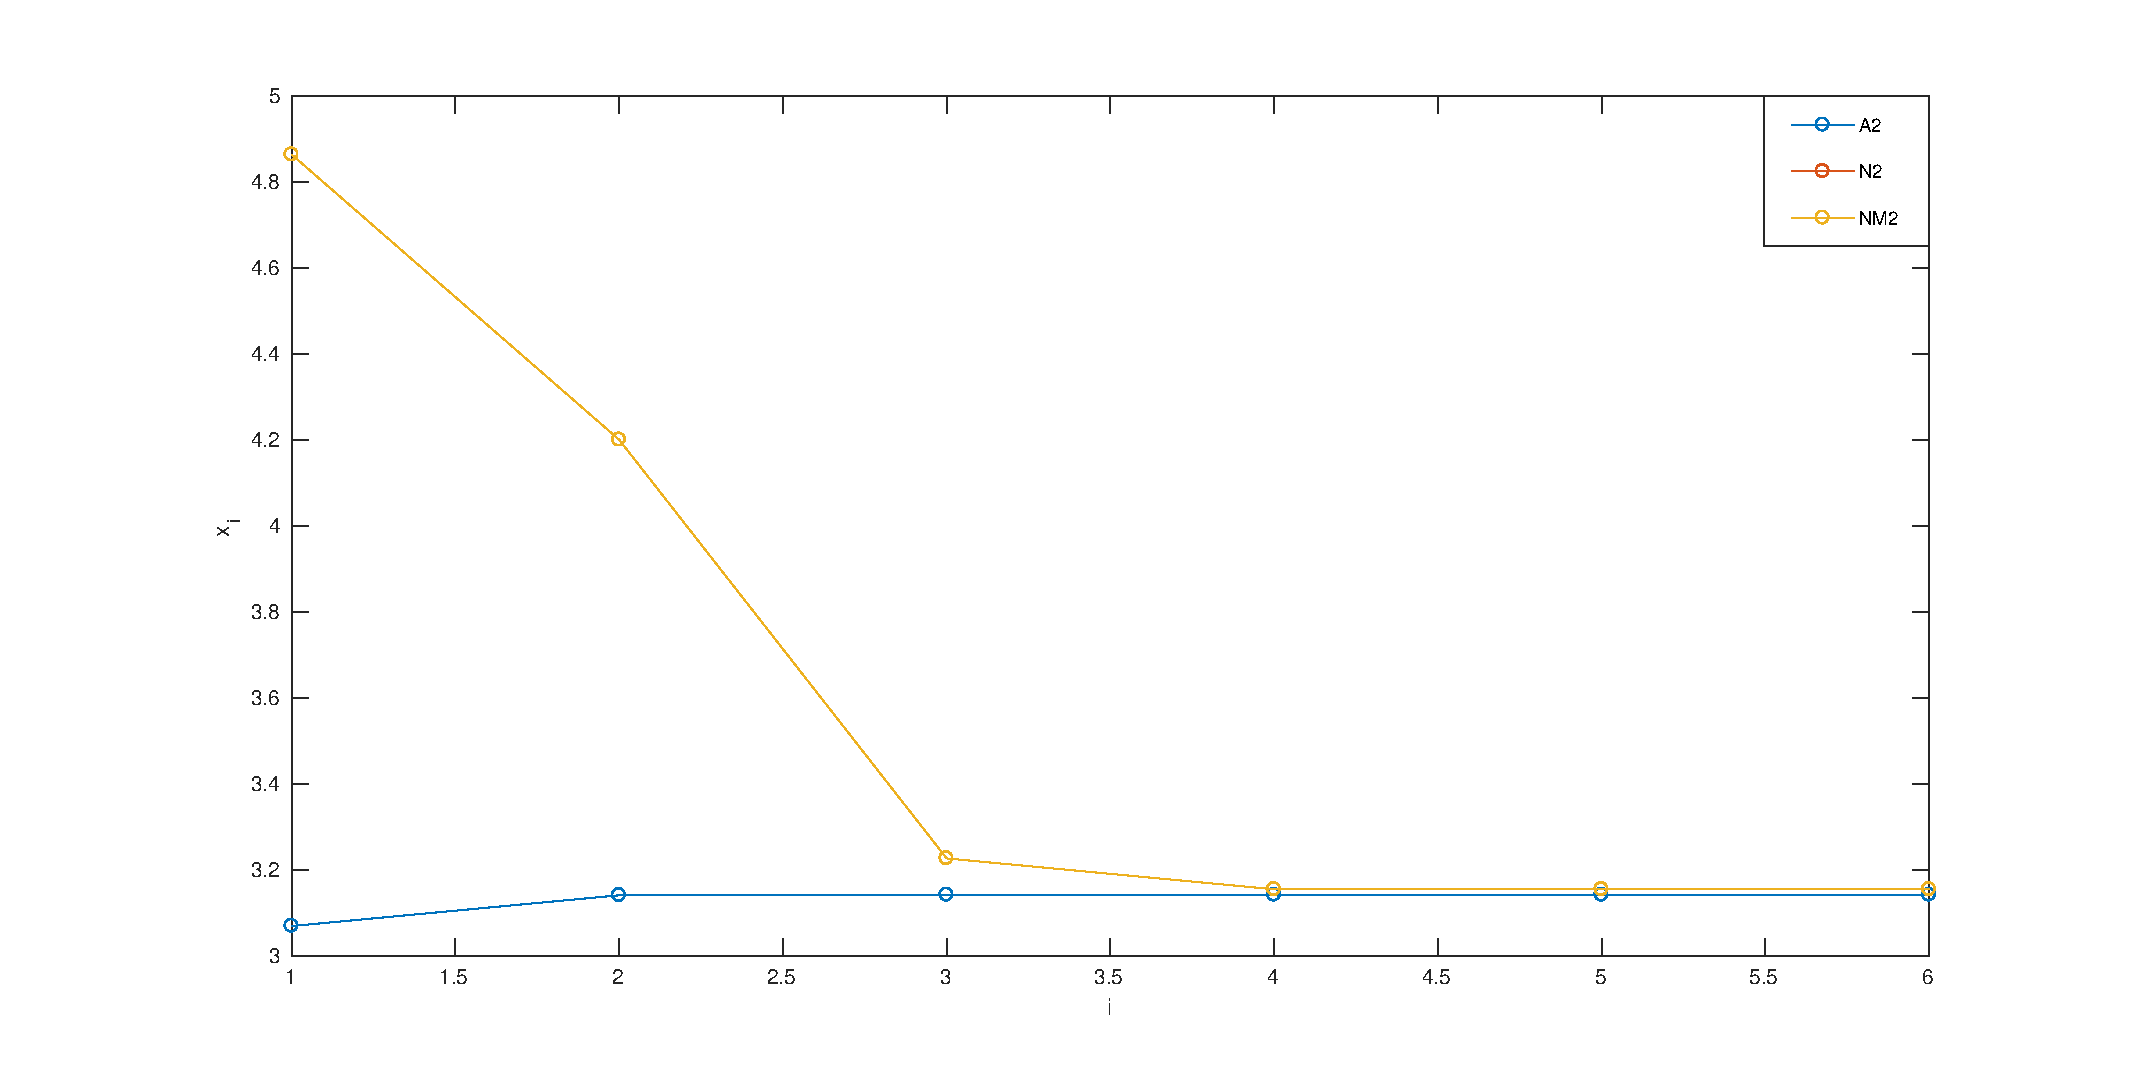
\includegraphics[left, width=210px]{plot/fes24b.eps}
\caption{Andamento del calcolo degli zeri della funzione $f_2(x) = (x-\pi)^{10} \cdot e^{2\cdot x}$ al variare della tolleranza}
\end{figure}
\end{flushleft}
\subsection{Esercizio 5}
Il metodo di bisezione \'e applicabile se la funzione \(f\) \'e
\begin{enumerate}

\item continua nell'intervallo \( [a,b] \)
\item tale che \( f(a)f(b)<0 \)

\end{enumerate}

Dal momento che lo zero delle funzioni \( f_1(x)=(x-\pi)^{10} \) e \( f_2(x)=e^{2x}(x-\pi)^{10} \) risulta essere in \( x=\pi \), ultilizzare come punto iniziale \( x_0 = 5 > \pi \) non porterebbe chiaramente alla determinazione dello zero ancor prima di valutare la regolarit\'a della funzione. 
Analizzando poi le due \( f \) si nota subito che \[
\nexists x | f_1(x)<0, \forall x \in \mathbb{R}, \]
\[
\nexists x | f_2(x)<0, \forall x \in \mathbb{R}.
\]


\begin {flushleft} Dal momento che queste sono funzioni esponeziali con minimo \(x_{min} = \pi \), risulta evidente come il suddetto metodo non sia applicabile. \end{flushleft}
 


\subsection{Esercizio 6}
\begin{flushleft}
Per poter costruire una tabella abbiamo scritto il seguente codice MatLab (lo script usa function definite a parte che è possibile vedere a pagina \pageref{functcap2}):
\lstinputlisting[language=Matlab]{cap_2/es6/es6.m}
Sotto forma tabellare rappresentiamo il numero di iterazioni effettuate dai 3 algoritmi (salvate nella matrice $iter$):

\begin{center}
\begin{tabular}{|c|c|c|c|}
\hline
$tol_x$ & Newton & Secanti & Corde \\
\hline
$10^{-1}$ & 2 & 3 & 2 \\
$10^{-2}$ & 3 & 3 & 8 \\
$10^{-3}$ & 3 & 4 & 15 \\
$10^{-4}$ & 3 & 5 & 22 \\
$10^{-5}$ & 4 & 5 & 28 \\
$10^{-6}$ & 4 & 5 & 35 \\
$10^{-7}$ & 4 & 5 & 42 \\
$10^{-8}$ & 4 & 6 & 48 \\
$10^{-9}$ & 4 & 6 & 55 \\
$10^{-10}$ & 5 & 6 & 62 \\
\hline
\end{tabular}
\end{center}
Questo risultato è possibile vederlo tramite il plot MatLab:
\begin{figure}[H]
\label{fes26}
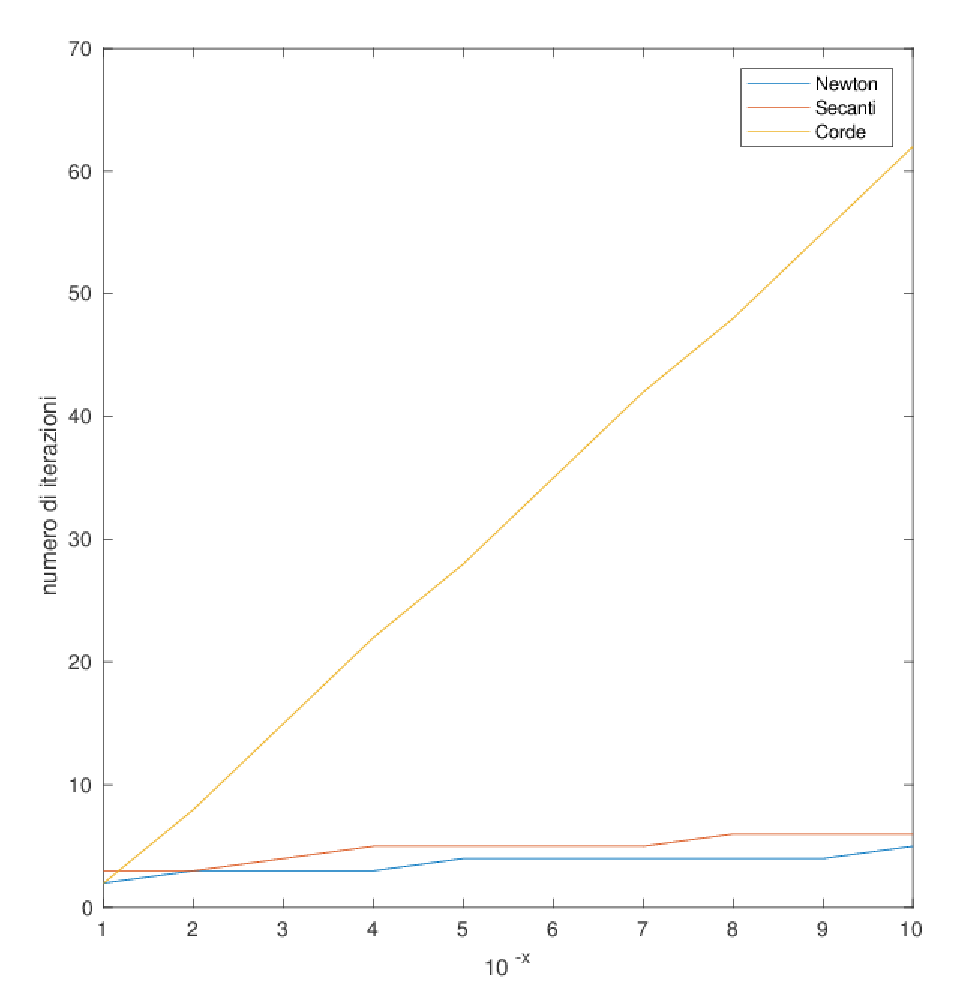
\includegraphics[width=480px, height=280px]{plot/fes26}
\caption{\texttt{\texttt{Andamento del numero delle iterazioni al decrescere della tolleranza per i metodi Newton, Secanti, Corde}}}
\end{figure}
Il numero di condizionamento del problema è dato da:
\[
k = \frac{1}{\big|f'(x^*)\big|}
\]
Per poterlo calcolare è necessario trovare la derivata della nostra funzione che è pari a:
\[
f'(x) = -1 - cos(x) + 5 \cdot sin(10\cdot x) - \frac{cos^2(10\cdot x)}{2}
\]
Essendo la radice della nostra funzione  $x^* = 0,488944$ il relativo numero di condizionamento è dato da:
\[
k = \frac{1}{\Big|f'(x^*)\Big|} = \frac{1}{\Big|f'(0,488944)\Big|} = \frac{1}{\Big|-4,27233\Big|} = \frac{1}{4,27233} = 0,234064
\]
questo significa che il problema è ben condizionato.
\end{flushleft}
\subsection{Esercizio 7}
\begin{flushleft}
Lo script usato è il seguente:
\lstinputlisting[language=MatLab]{cap_2/es7/es7.m}
\lstinputlisting[language=matlab]{cap_2/bisect.m}
Il numero di iterazioni del metodo di bisezione risultanti sono:

\begin{center}
\begin{tabular}{|c|c|c|c|}
\hline
$tol_x$ & bisezione \\
\hline
$10^{-1}$ & 2 \\
$10^{-2}$ & 7 \\
$10^{-3}$ & 10 \\
$10^{-4}$ & 14 \\
$10^{-5}$ & 17 \\
$10^{-6}$ & 20 \\
$10^{-7}$ & 24 \\
$10^{-8}$ & 27 \\
$10^{-9}$ & 30 \\
$10^{-10}$ & 34 \\
\hline
\end{tabular}
\end{center}

Si può vedere dal grafico l'andamento dei vari metodi usati nel seguente plot MatLab:
\begin{figure}[H]
\label{fes27}
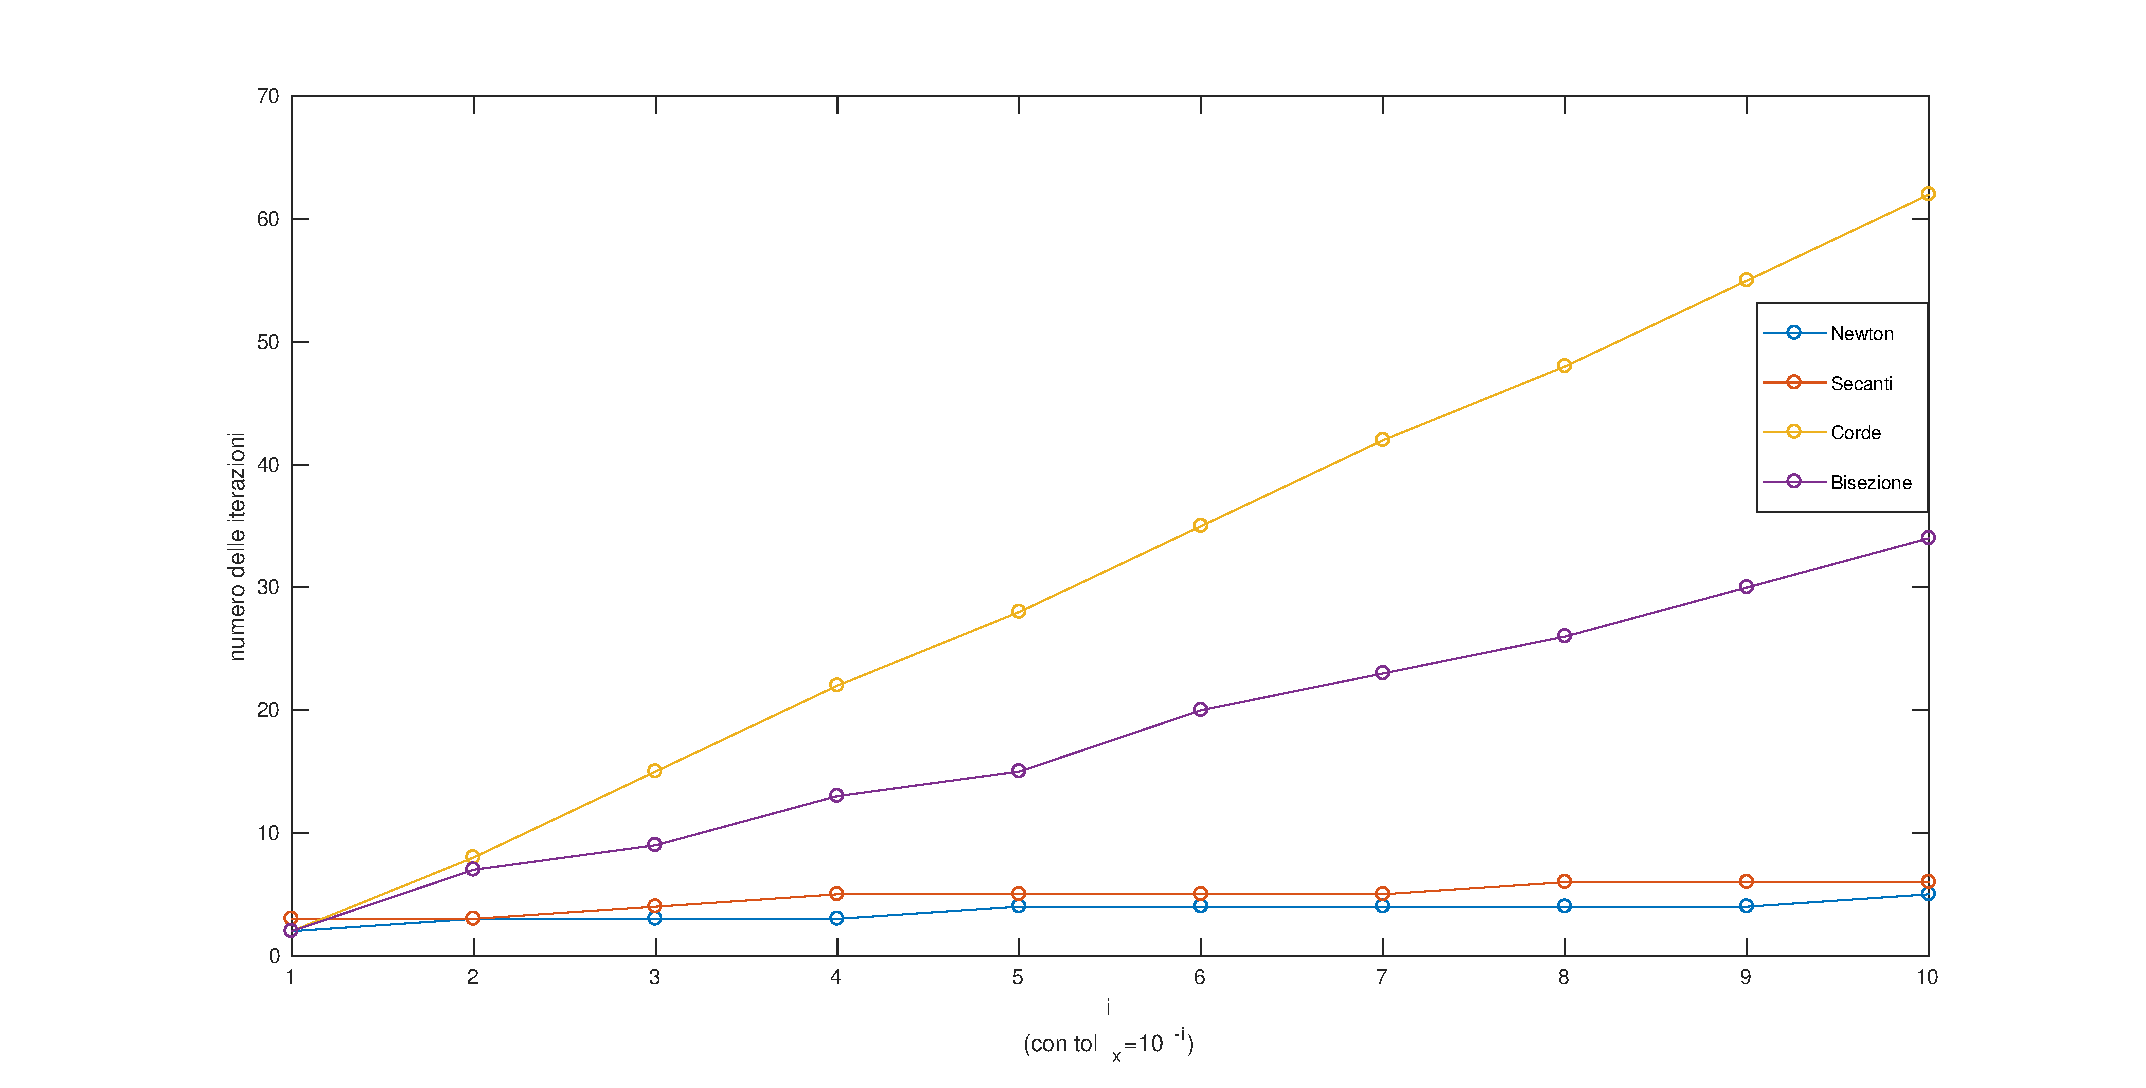
\includegraphics[width=480px, height=280px]{plot/fes27}
\caption{\texttt{Aggiunta dell'andamento del metodo di Bisezione rispetto ai precedenti metodi}}
\end{figure}

\end{flushleft}
\subsection{Esercizio 8}
\lstinputlisting[language=Matlab]{cap_2/es8/es8.m}

Essendo \[f'(x)=10(x-\pi)^{10x}(\frac{x}{x-\pi}+\ln{(x-\pi)})\]
E dato che quest'ultima contiene $ln(x - \pi)$, il cui dominio \'e \( \{ \forall x \in \mathbb{R} | x > \pi \}\), il metodo non potrà convergere per valori di $x_0 \leq \pi$

\newpage
\subsection{Funzioni MatLab Usate}
\label{functcap2}
\subsubsection{Metodo Newton per $\sqrt{\alpha}$}
\lstinputlisting[language=matlab]{cap_2/NewtonSqrt.m}
\subsubsection{Metodo Newton per $\sqrt[n]{\alpha}$}
\lstinputlisting[language=matlab]{cap_2/NewtonSqrtN.m}
\subsubsection{Metodo delle secanti per $\sqrt{\alpha}$}
\lstinputlisting[language=matlab]{cap_2/SecSqrt.m}
\subsubsection{Metodo di Newton}
\lstinputlisting[language=matlab]{cap_2/Newton.m}
\subsubsection{Metodo di Newton Modificato}
\lstinputlisting[language=matlab]{cap_2/NewtonMod.m}
\subsubsection{Metodo di accelerazione di Aitken}
\lstinputlisting[language=matlab]{cap_2/Aitken.m}
\subsubsection{Metodo delle secanti}
\lstinputlisting[language=matlab]{cap_2/secanti.m}
\subsubsection{Metodo delle corde}
\lstinputlisting[language=matlab]{cap_2/corde.m}
\subsubsection{Metodo della bisezione}
\lstinputlisting[language=matlab]{cap_2/bisect.m}
\section{Capitolo 3}
\underline{Le funzioni usate nei codici seguenti sono in fondo al capitolo}
\subsection{Esercizio 1}
Una matrice \( L \in M_{n \times n} \) si dice triangolare inferiore se \( l_{i,j}=0, \forall i<j \) con \(i,j = 1...n \) ed \( l_{i,j} \in L \).
\\
Date due matrici triangolari inferiori \( L,K \in M_{n \times n} \) la loro somma sar\'a di nuovo una matrice traingolare inferiore \( N \in M_{n \times n} \):
\[
 \forall i<j, \hspace{5pt} l_{i,j} + k_{i,j} = 0 + 0 = 0. 
\]
\\
Una matrice \( U \in M_{n \times n} \) si dice triangolare superiore se \( u_{i,j}=0, \forall i>j \) con \(i,j = 1...n \) ed \( u_{i,j} \in U \).
Date due matrici triangolari superiori  \( U,W \in M_{n \times n} \)  il loro prodotto  \( Z \in M_{n \times n} \):
\[
z_{i,j} = \sum_{k=1}^n u_{i,k} w_{k,j}, \hspace{35pt} \forall i,j \in [1,..,n].
\]
sar\'a di nuovo una matrice triangolare superiore, dal momento che 
\[
z_{i,j} =  \sum_{k=1}^n u_{i,k} w_{k,j} =  \underbrace{ \sum_{k=1}^{i-1} u_{i,k} w_{k,j} }_\text{=0 per k<i}  + \sum_{k=i}^n u_{i,k} w_{k,j} = \sum_{k=i}^n u_{i,k} w_{k,j}.
\]
Dal momento che in quest'ultimo termine abbiamo \( k \geq i \) se \( i>j \) allora \( k>j \), da cui la definizione di matrice triangolare superiore.

\subsection{Esercizio 2}
Se $U,W \in M_{n \times n}$ sono matrici triangolari superiori a diagonale unitaria si ha che gli elementi diagonali della matrice $Z=UW$ saranno calcolati come
\[
z_{i,i} = \sum_{k=i}^{i} u_{i,i}w_{i,i} = 1 \cdots 1 = 1.
\]
Quindi, riallacciandosi alla dimostrazione dell'esercizio \textbf{3.1} si ha che la matrice $Z$ \'e triangolare superiore a diagonale unitaria.
$symbol$

\subsection{Esercizio 3}
Sia $A \in M_{n \times n}$ una matrice triangolare superiore non singolare.\\
Se $A$ \'e invertibile allora pu\'o essere scritta come $A=D(\mathit{I_n}+U)$ dove $D$ \'e una matrice diagonale per cui vale $diag(D)=diag(A)$, $\mathit{I_n}$ \'e la matrice identit\'a ed $U$ \'e una matrice triangolare strettamente superiore ($diag(U)=0$).\\
Per le propriet\'a delle matrici triangolari strettamente superiori si ha che $U^n = 0$ (ovvero che la matrice $U$ \'e nilpotente), mentre per le propriet\'a delle matrici diagonali si ha che $D^{-1}$ \'e ancora una matrice diagonale.
\\
Volendo provare che $A^{-1}=(\mathit{I_n}+U)^{-1}D^{-1}$ espandiamo in serie $ (\mathit{I_n}+U)^{-1}$:
\[
(\mathit{I_n}+U)^{-1}=\mathit{I_n}-U+U^2-...+(-1)^{n-1}U^{n-1}.
\]
Essendo questa una serie di somme e prodotti di matrici triangolari superiori la matrice inversa $A^{-1}$ sar\'a in generale una matrice triangolare superiore.
\subsection{Esercizio 4}
L'eliminazione nella prima colonna richiede $n$ somme ed $n$ prodotti per $n-1$ righe, quindi in totale $(n+n)(n-1) = 2n(n-1)$ \texttt{flops}. L'eliminazione della seconda richiede $n-1$ somme ed $n-1$ prodotti per $n-2$ righe, quindi in totale $[(n-1)+(n-1)](n-2) = 2(n-1)(n-2)$ \texttt{flops}.\\
Procedendo per induzione si ha che il numero totale di operazioni \'e
\[
\sum_{i=0}^{n} 2(n-i)(n-i+1). \hspace{50pt} (1)
\]
Operando la sostituzione $y \doteq n-i+1$ si ha che la (1) diviene :

\[
2 \sum_{j=0}^{n-1} j(j-1) = 2 \sum_{j=0}^{n-1}j^2 + j = 2 ( \frac{1}{3}n^3 - \frac{1}{3}n)
\]
Asintoticamente quindi proprio $\frac{2}{3}n^3$ \texttt{flops}.


\subsection{Esercizio 5}
\begin{flushleft}
L'algoritmo di fattorizzazione LU con pivoting parziale da noi implementato è il seguente:
\lstinputlisting[language=matlab]{cap_3/factLUP.m}
è possibile vedere il funzionamento di questa function nell'esercizio 14 a pagina \pageref{es314}.
\end{flushleft}
\subsection{Esercizio 6}
\lstinputlisting[language=Matlab]{cap_3/solveLinearLUP.m}

\subsection{Esercizio 7}
Sia $\mathbf{v} \in \mathbb{R}^n| \mathbf{v} \neq \mathbf{0}$ e $A \in M_{n \times n}$.
$A$ si dice sdp (simmetrica definita positiva) se \'e simmetrica ($A$=$A^T$) e se $\mathbf{v}^TA\mathbf{v} > 0.$
Equivalentemente una matrice si dice sdp se \'e simmetrica ed i suoi autovalori sono $> 0.$
Inoltre una matrice $B \in M_{n \times n}$ si dice nonsingolare se $\det{B} \neq 0.$
\\
Dal momento che il polinomio caratteristico \'e invariante per similitudine le matrici quadrate $A$ ed $A^T$ hanno gli stessi autovalori.
Inoltre le matrici $A^TA$ ed $AA^T$ sono simmetriche.
Vale poi $\det{(A^TA)} = \det{(AA^T)} = \det{A}\det{A^T} = (\det{A})^2.$

finisco stase

\subsection{Esercizio 8}
Se $A \in M_{m \times n}$ con $m \geq n = rank(A)$ allora diremo che $A$ ha rango massimo.
\\
Questo comporta che la matrice sia invertibile, ovvero che il suo determinante $\det(A) \neq 0$. La matrice \'e quindi nonsingolare e di conseguenza simmetrica definita positiva, dalla dimostrazione dell'esercizio \textbf{3.7}.
\subsection{Esercizio 9}
Si ha ovviamente che 
\[
A = \frac{1}{2}(A+A^T) + \frac{1}{2}(A-A^T)=\frac{1}{2}A + \frac{1}{2}A^T + \frac{1}{2}A - \frac{1}{2}A^T
\]
\\
Definendo $A_s \doteq \frac{1}{2}(A+A^T)$ si mostra come $A_s = A_s^T$ infatti
\[
\frac{1}{2}(A+A^T) = [ \frac{1}{2}(A+A^T)]^T = \frac{1}{2}(A+A^T)^T = \frac{1}{2}(A^T+(A^T)^T) = \frac{1}{2}(A+A^T)^T.
\]
\\
Da cui $A_s$ \'e detta parte \textbf{simmetrica} di $A$.
\\
Definendo $A_a \doteq \frac{1}{2}(A-A^T)$ si mostra come $A_a = -A_a^T$ infatti
\[
\frac{1}{2}(A-A^T) = -\frac{1}{2}(A-A^T)^T = -\frac{1}{2}(A^T-(A^T)^T) = -\frac{1}{2}(A^T-A) = \frac{1}{2}(A-A^T).
\]
Da cui $A_a$ \'e detta parte \textbf{antisimmetrica} di $A$.
\\
Dato poi un generico vettore $\mathbf{x} \in \mathbf{R}^n$ si ha che $\mathbf{x}^TA\mathbf{x} = \mathbf{x}^TA_s\mathbf{x}$ infatti
\[
\mathbf{x}^TA\mathbf{x} = \mathbf{x}^T(A_s + A_a)\mathbf{x} = \mathbf{x}^TA_s\mathbf{x} + \mathbf{x}^TA_a\mathbf{x} = \frac{1}{2}(\mathbf{x}^TA\mathbf{x} + \mathbf{x}^TA^T\mathbf{x}) + \frac{1}{2}(\mathbf{x}^TA\mathbf{x} - \mathbf{x}^TA^T\mathbf{x}).
\]
Analizzando l'ultimo termine $\frac{1}{2}(\mathbf{x}^TA\mathbf{x} - \mathbf{x}^TA^T\mathbf{x})$ si nota come
\[ \frac{1}{2}(\mathbf{x}^TA\mathbf{x} - \mathbf{x}^TA^T\mathbf{x}) = \frac{1}{2}(\mathbf{x}^TA\mathbf{x} - (A\mathbf{x})^T\mathbf{x})=0
\]
\\
dal momento che, definendo $A\mathbf{x}=\mathbf{y}$ si ha $\mathbf{x}^T\mathbf{y}= \mathbf{y}^T\mathbf{x}.$
Da cui la tesi.

\subsection{Esercizio 10}
L'algoritmo esegue $i-1$ somme di due prodotti, una sottrazione ed una divisione per un costo totale di $2(i-1)+2$ \texttt{flops}. Essendo la matrice triangolare, per ogni colonna eseguir\'a il calcolo $n-i$ volte.
\\
Quindi
\[
\sum_{i=1}^{n} 2i(n-i) = 2(n \sum_{i=1}^{n}i - \sum_{i=1}^{n} i^2) = 2n\frac{n(n+1)}{2} - 2\frac{n(n+1)(2n+1)}{6} = n^3 + n^2 - \frac{2n^3 + 3n^2 + n}{3} = \frac{n^3}{3} - \frac{n}{3} \approx \frac{n^3}{3}.
\]

\subsection{Esercizio 11}
\lstinputlisting[language=Matlab]{cap_3/es11/fattorizzaLDLt.m}
\subsection{Esercizio 12}
\begin{flushleft}
Supponendo che in ingresso si abbiano le matrici di fattorizzazione $LDL^T$ di una qualsiasi matrice $M \in \mathbb{R}^{n\times n}$ SDP, rispettivamente:
\begin{itemize}
    \item L matrice triangolare inferiore a diagonale unitaria
    \item D matrice diagonale con elementi diagonali positivi
\end{itemize}
e b vettore dei termini noti, è possibile scrivere la function linLDL che risolve sistemi lineari:
\lstinputlisting[language=matlab]{cap_3/linLDLT.m}
\end{flushleft}
\subsection{Esercizio 13}
\begin{flushleft}
Per verificarlo abbiamo usato il seguente codice MatLab:
\lstinputlisting[language=Matlab]{cap_3/es13/es13.m}
Che restituisce l'output:
\begin{lstlisting}[language=matlab, basicstyle = \small]
A1 =
     1     1     1     1
     1     2     2     2
     1     2     3     3
     1     2     3     4
L1 =
     1     0     0     0
     1     1     0     0
     1     1     1     0
     1     1     1     1
D1 =
     1     0     0     0
     0     1     0     0
     0     0     1     0
     0     0     0     1
     
A2 =
     1     1     1     1
     1     2     2     2
     1     2     3     3
     1     2     3     2
Error using factLDLT (line 14)
[Errore] La matrice non e' SDP
Error in es13 (line 6)
[L2,D2] = factLDLT(A2) 
\end{lstlisting}
L'output è molto chiaro, la seconda matrice $A_{2}$ non può essere fattorizzata $LDL^T$ di conseguenza non è $SDP$.
\end{flushleft}


\subsection{Esercizio 14}
\label{es314}
\begin{flushleft}
Nel primo caso abbiamo usato la matrice $A\in M^{3\times 3}$ con elementi:
\[ 
A =
\begin{pmatrix}
    0 & -3 &  8 \\
   -1  &  8  &  7 \\
    1  &  3  &  0 \\
\end{pmatrix}
\]
e il vettore dei termini noti $b\in \mathbb{R}^3$ con valori:
\[
b = \begin{pmatrix}
    3.1416 \\
    1.1618 \\
    2.7183 \\
\end{pmatrix}
\]
Nel secondo caso abbiamo usato la matrice $A\in M^{3\times 3}$ con elementi:
\[ 
A =
\begin{pmatrix}
    14 & 5 &  2 \\
    5 &  8  &  1 \\
    2  &  1  &  4 \\
\end{pmatrix}
\]
e il vettore dei termini noti $b\in \mathbb{R}^3$ con valori:
\[
b = \begin{pmatrix}
    3.1416 \\
    1.1618 \\
    2.7183 \\
\end{pmatrix}
\]
Usando il codice MatLab sottostante è possibile risolvere questi 2 esempi:
\lstinputlisting[language=Matlab]{cap_3/es14/es14.m}
Il codice sopra restituisce l'output:
\begin{figure}[H]
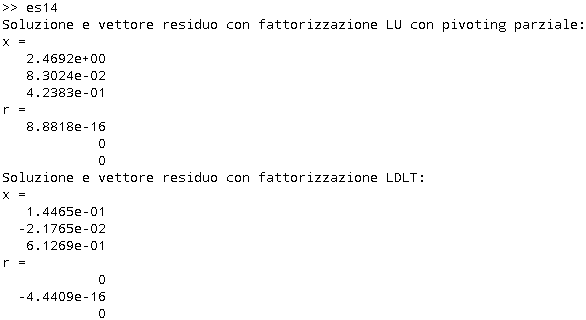
\includegraphics[left, width=300px]{cap_3/es14/es314.png}
\end{figure}
\end{flushleft}
\subsection{Esercizio 15}
\begin{flushleft}
\lstinputlisting[language=Matlab]{cap_3/es15/es15.m}
Il codice MatLab sopra restituisce in output:
\begin{lstlisting}[language=matlab, basicstyle = \small]
ans =
    101.000000000000e+000
ans =
    101.000000000000e+000
Warning: Matrix is close to singular or badly scaled.
Results may be inaccurate. RCOND =  9.801980e-21. 
> In cond (line 46)
  In es15 (line 7) 
ans =
    102.020202020202e+018
\end{lstlisting}
Analiticamente abbiamo che $\rVert A \rVert_{\infty} = \rVert A \rVert_1 = 101$, come \'e possibile verificare attraverso l'istruzione norm di Matlab.
Per quanto riguarda il calcolo del numero di condizionamento $k_{\infty}(A)$ abbiamo che, andando a calcolare l'inversa, gli elementi della matrice crescono di 2 ordini di grandezza per ogni riga, arrivando ad avere valori prossimi a $10^{18}$. Questo implica che $\rVert A^{-1} \rVert_{\infty}>10^{20}$ per cui possiamo affermare che il problema \'e malcondizionato.
La verifica con l'istruzione cond di Matlab restituisce un warning in cui avverte che $RCOND=9.801980e-21$, confermando quanto appena detto.
\end{flushleft}
\subsection{Esercizio 16}
\lstinputlisting[language=Matlab]{cap_3/es16/es16.m}

\subsection{Esercizio 17}
\begin{flushleft}
L'algoritmo di fattorizzazione QR, mediante metodo di householder, da noi implementato è il seguente:
\lstinputlisting[language=matlab]{cap_3/factQRH.m}
è possibile vedere il funzionamento di questa function nell'esercizio 19 a pagina \pageref{es319}.
\end{flushleft}
\subsection{Esercizio 18}
\lstinputlisting[language=Matlab]{cap_3/solveQR.m}

\subsection{Esercizio 19}
\label{es319}
\begin{flushleft}
Il codice usato è:
\lstinputlisting[language=Matlab]{cap_3/es19/es19.m}
che ha generato questo risultato:
\begin{figure}[h]
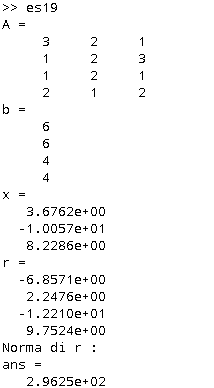
\includegraphics[left, width=300px]{cap_3/es19/es319}
\end{figure}
\end{flushleft}

\subsection{Esercizio 20}
Risolviamo il sistema di equazioni non lineari applicando il metodo di Newton.
La funzione data è \[F(x_1, x_2)= \begin{cases}x_2-cos(x_1)\\ x_1x_2 -1/2\end{cases}\]
Vogliamo trovare $F(x_1, x_2)=0$ partendo da $x_1(0) = 1\mbox{, } x_2(0) = 1$\\
Troviamo quindi il Jacobiano della funzione: \( J=\begin{pmatrix} sin(x_1) & 1  \\\ x_1 & x_2 \end{pmatrix} \)\\
Applicando il metodo di Newton si va a risolvere:
$\begin{cases} J_F(\underline{x}^{(k)})\underline{d}^{(k)}=-F(\underline{x}^{(k)}) \\ \quad \underline{x}^{(k+1)}=\underline{x}^{(k)}+\underline{d}^{(k)} \end{cases}$\\
Troviamo quindi: $x_1 = 0.6100 \mbox{ e } x_2 =0.8196$

Il codice matlab per il calcolo del minimo è:
\lstinputlisting[language=Matlab]{cap_3/es20/es20.m}

Il codice matlab per la risoluzione di sistemi di equazioni non lineari mediante Newton è:
\lstinputlisting[language=Matlab]{cap_3/NewtonNL.m}

\begin{tabular}{l|c|r}
i & $x_1,x_2$ & norma dell'incremento \\
\hline
1 & 0.7458, 0.7542 & 0.5001 \\
2 & 0.5531, 0.8653 & 0.3145 \\
3 & 0.6042, 0.8241 & 0.0929 \\
4 & 0.6100, 0.8197 & 0.0102 \\
5 & 0.6100, 0.8196 & 0.00013 \\ 


\end{tabular}

\subsection{Esercizio 21}
Un punto stazionario $(\hat{x_1}, \hat{x_2})$ è tale per cui $J(\hat{x_1},\hat{x_2})=0$. Si ottiene quindi il sistema non lineare:
$$F(\underline{x})=\underline{0}\mbox{ con }F=\begin{pmatrix}\frac{\partial f}{\partial x_1}\\\frac{\partial f}{\partial x_2}\end{pmatrix}=\begin{pmatrix}4x_1^3+2x_1+x_2\\x_1+2x_2-2\end{pmatrix}.$$
Troviamo il Jacobiano della funzione: \( J=\begin{pmatrix} 12x_1^2+2 & 1  \\\ 1 & 2 \end{pmatrix} \)\\

Troviamo quindi $$\min{f(x_1,x_2)}\approx -0.2573\mbox{ in }(0.4433, -1.2217).$$


Il codice matlab per il calcolo del minimo è:
\lstinputlisting[language=Matlab]{cap_3/es21/es21.m}

\subsection{Funzioni MatLab Usate}
\label{functcap3}
\begin{flushleft}
\subsubsection{Fattorizzazioni}
\begin{itemize}
    \item \texttt{Fattorizzazione LU con pivoting parziale}
\lstinputlisting[language=Matlab]{cap_3/factLUP.m}
    \item \texttt{Fattorizzazione LDLT}
\lstinputlisting[language=Matlab]{cap_3/factLDLT.m}
    \item \texttt{Fattorizzazione QR mediante metodo di Householder}
\lstinputlisting[language=Matlab]{cap_3/factQRH.m}
\end{itemize}
\subsubsection{Function per la risoluzione sistemi lineari}
\begin{itemize}
    \item \texttt{Calcolo matrice trinagolare inferiore}
\lstinputlisting[language=Matlab]{cap_3/triInf.m}
    \item \texttt{Calcolo matrice trinagolare superiore}
\lstinputlisting[language=Matlab]{cap_3/triSup.m}
    \item \texttt{Calcolo diagonale principale}
\lstinputlisting[language=Matlab]{cap_3/triSup.m}
\end{itemize}
\subsubsection{Risoluzione sistemi lineari, sovradeterminati e non lineari}
\begin{itemize}
    \item \texttt{Risoluzione sistema lineare con matrice matrice dei coefficienti fattorizzata LUP}
\lstinputlisting[language=Matlab]{cap_3/linLUP.m}
    \item \texttt{Risoluzione sistema lineare con matrice matrice dei coefficienti fattorizzata LDLT}
\lstinputlisting[language=Matlab]{cap_3/linLDLT.m}
    \item \texttt{Risoluzione sistema lineare sovradeterminato con matrice dei coefficienti fattorizzata QRH}
\lstinputlisting[language=Matlab]{cap_3/solveQRH.m}
    \item \texttt{Risoluzione sistema non lineare con metodo di Newton}
\lstinputlisting[language=Matlab]{cap_3/nonLinearNewton.m}
\end{itemize}
\end{flushleft}
\newpage
\pagenumbering{roman}
\section{\textbf{Grafici}}
\begin{figure}[h]
\caption{Esercizio 1.4}
\label{fes14}
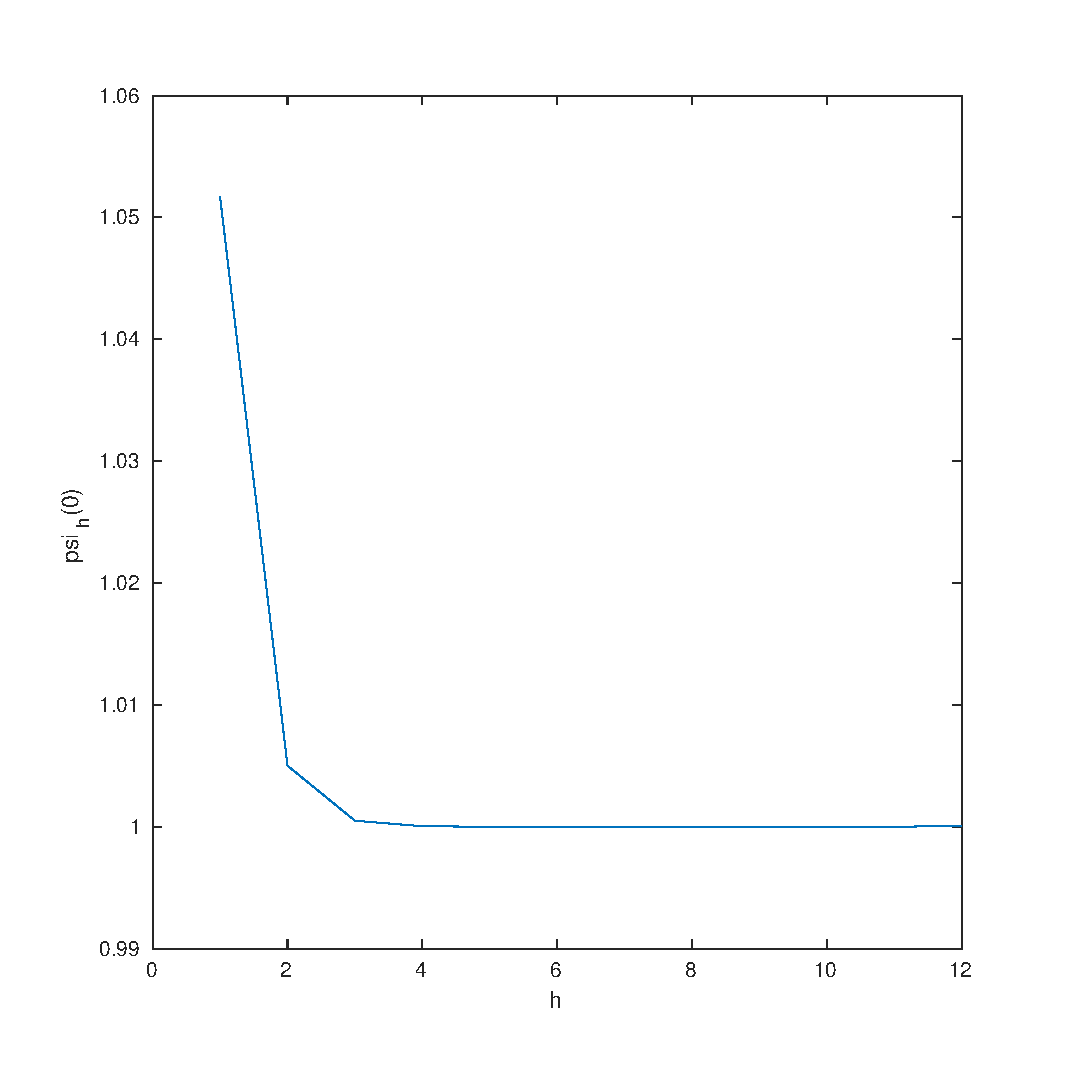
\includegraphics[width=\textwidth]{plot/fes14}
\end{figure}
\begin{figure}[h]
\caption{Esercizio 1.13}
\label{fes113}
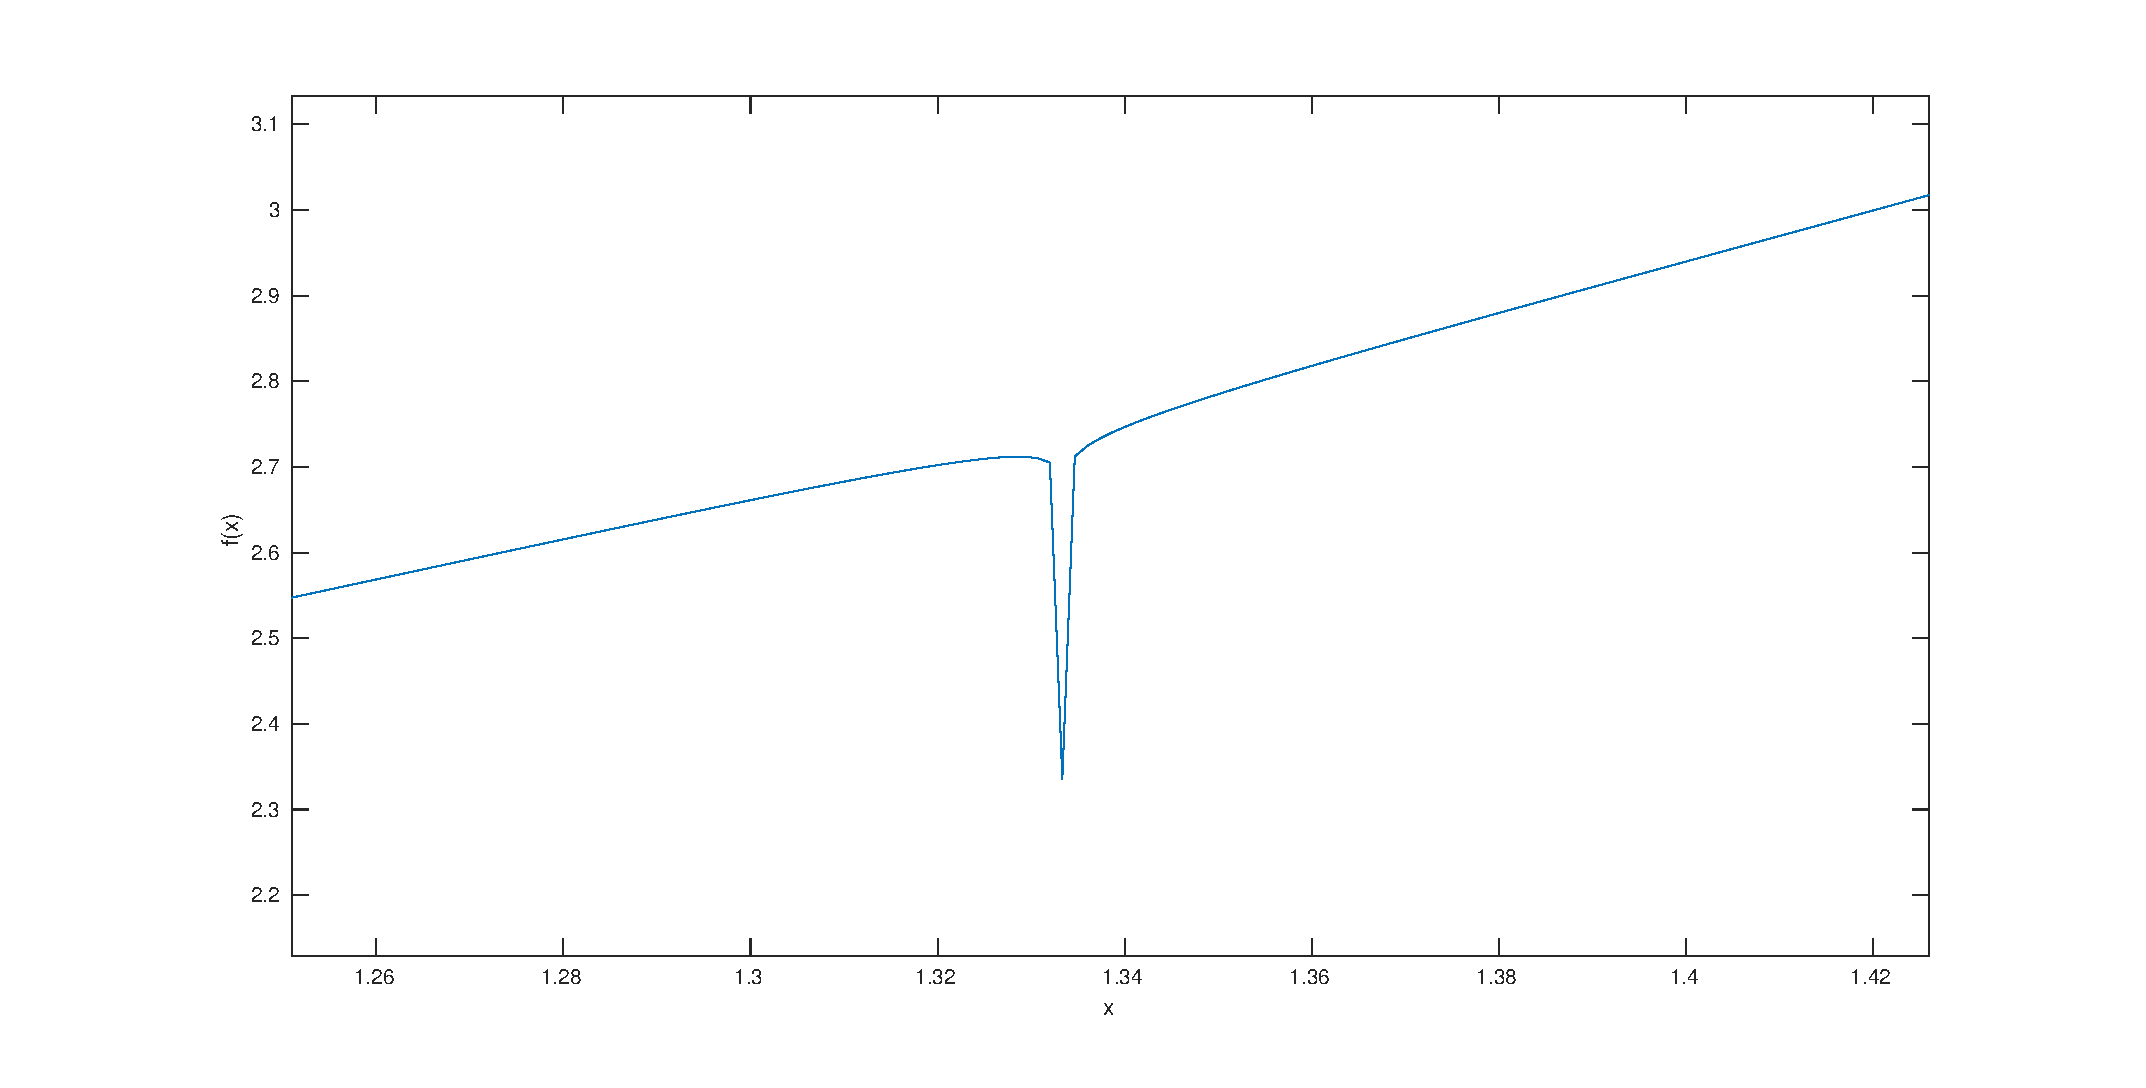
\includegraphics[width=\textwidth]{plot/fes113}
\end{figure}
\begin{figure}[h]
\caption{Runge Chebyshev}
\label{RungeChe}
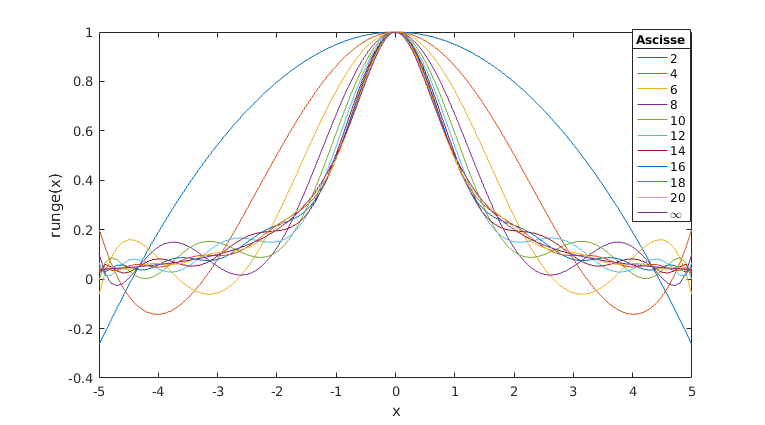
\includegraphics[width=\textwidth]{plot/Runge_cheb}
\end{figure}
\begin{figure}[h]
\caption{Runge Chebyshev Errori}
\label{RungeCheErr}
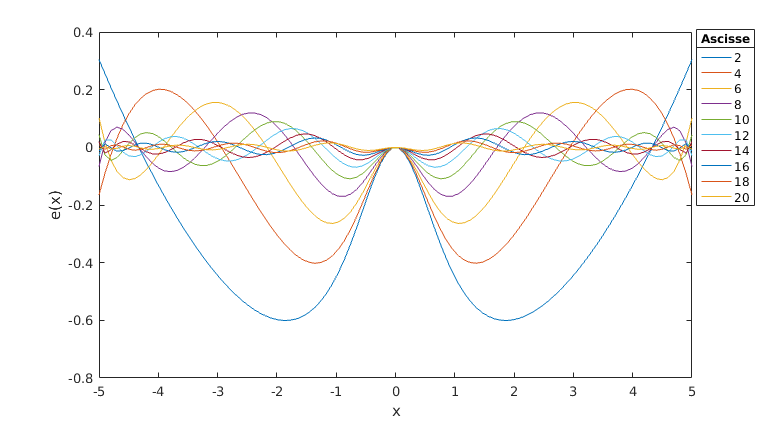
\includegraphics[width=\textwidth]{plot/Runge_cheb_err}
\end{figure}
\begin{figure}[h]
\caption{Runge con ascisse equidistanti}
\label{RungeEq}
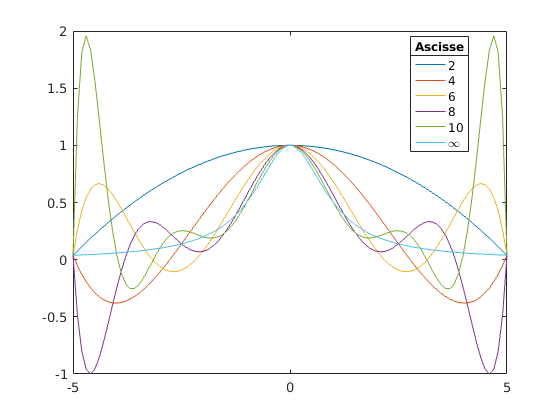
\includegraphics[width=\textwidth]{plot/Runge_equi}
\end{figure}
\begin{figure}[h]
\caption{Runge con ascisse equidistanti errori}
\label{RungeEqErr}
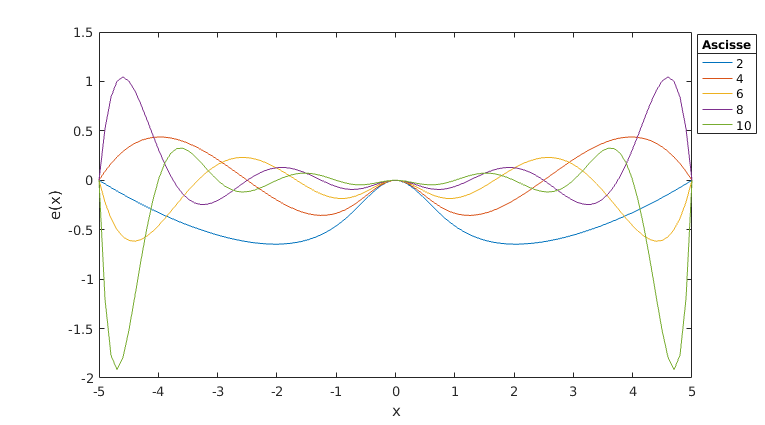
\includegraphics[width=\textwidth]{plot/Runge_equi_err}
\end{figure}
\begin{figure}[h]
\caption{Funzione xsinx Chebyshev}
\label{SinChe}
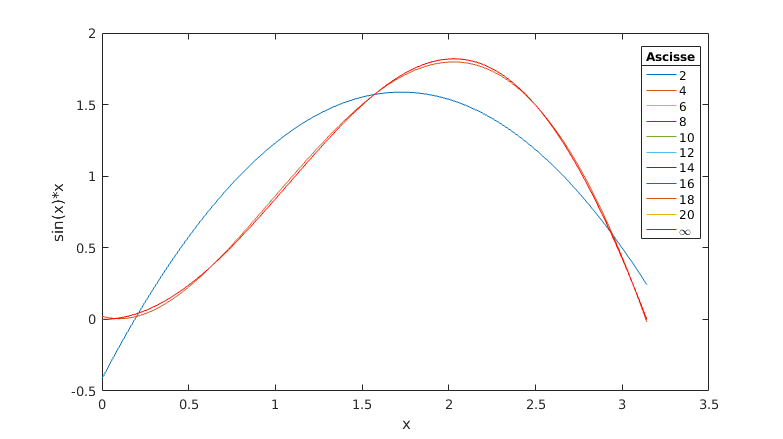
\includegraphics[width=\textwidth]{plot/Sin_cheb}
\end{figure}
\begin{figure}[h]
\caption{Funzione xsinx Chebyshev errori}
\label{SinCheErr}
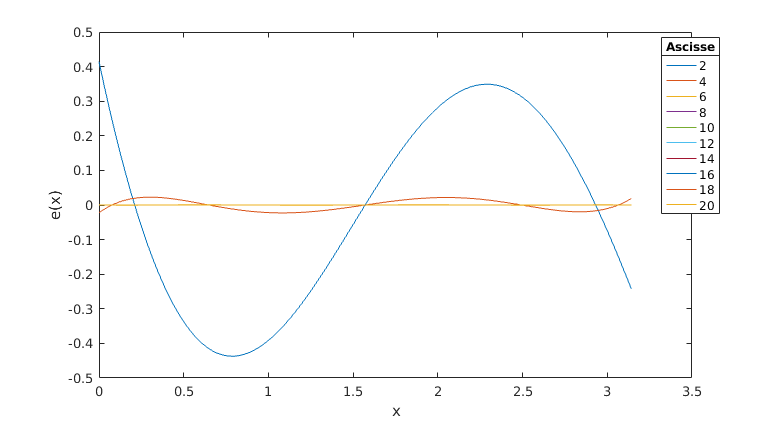
\includegraphics[width=\textwidth]{plot/Sin_cheb_Err}
\end{figure}
\begin{figure}[h]
\caption{Funzione xsinx ascisse equidistanti}
\label{SinEq}
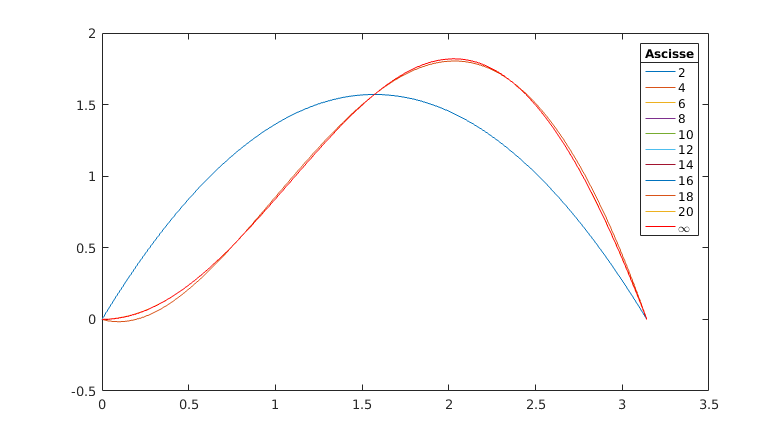
\includegraphics[width=\textwidth]{plot/Sin_equi}
\end{figure}
\begin{figure}[h]
\caption{Funzione xsinx ascisse equidistanti errori}
\label{SinEqErr}
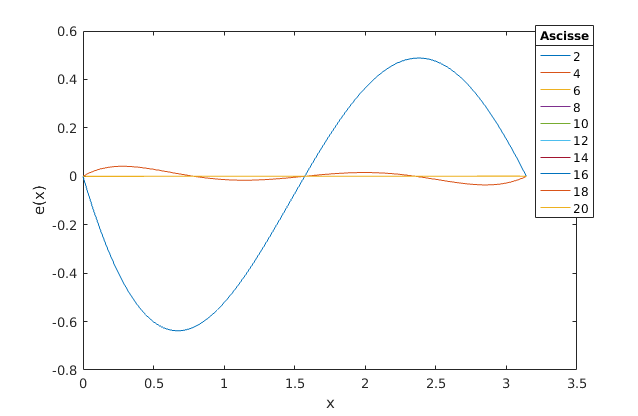
\includegraphics[width=\textwidth]{plot/Sin_equi_err}
\end{figure}
\begin{figure}[h]
\caption{Runge not-a-knot}
\label{runge_nak}
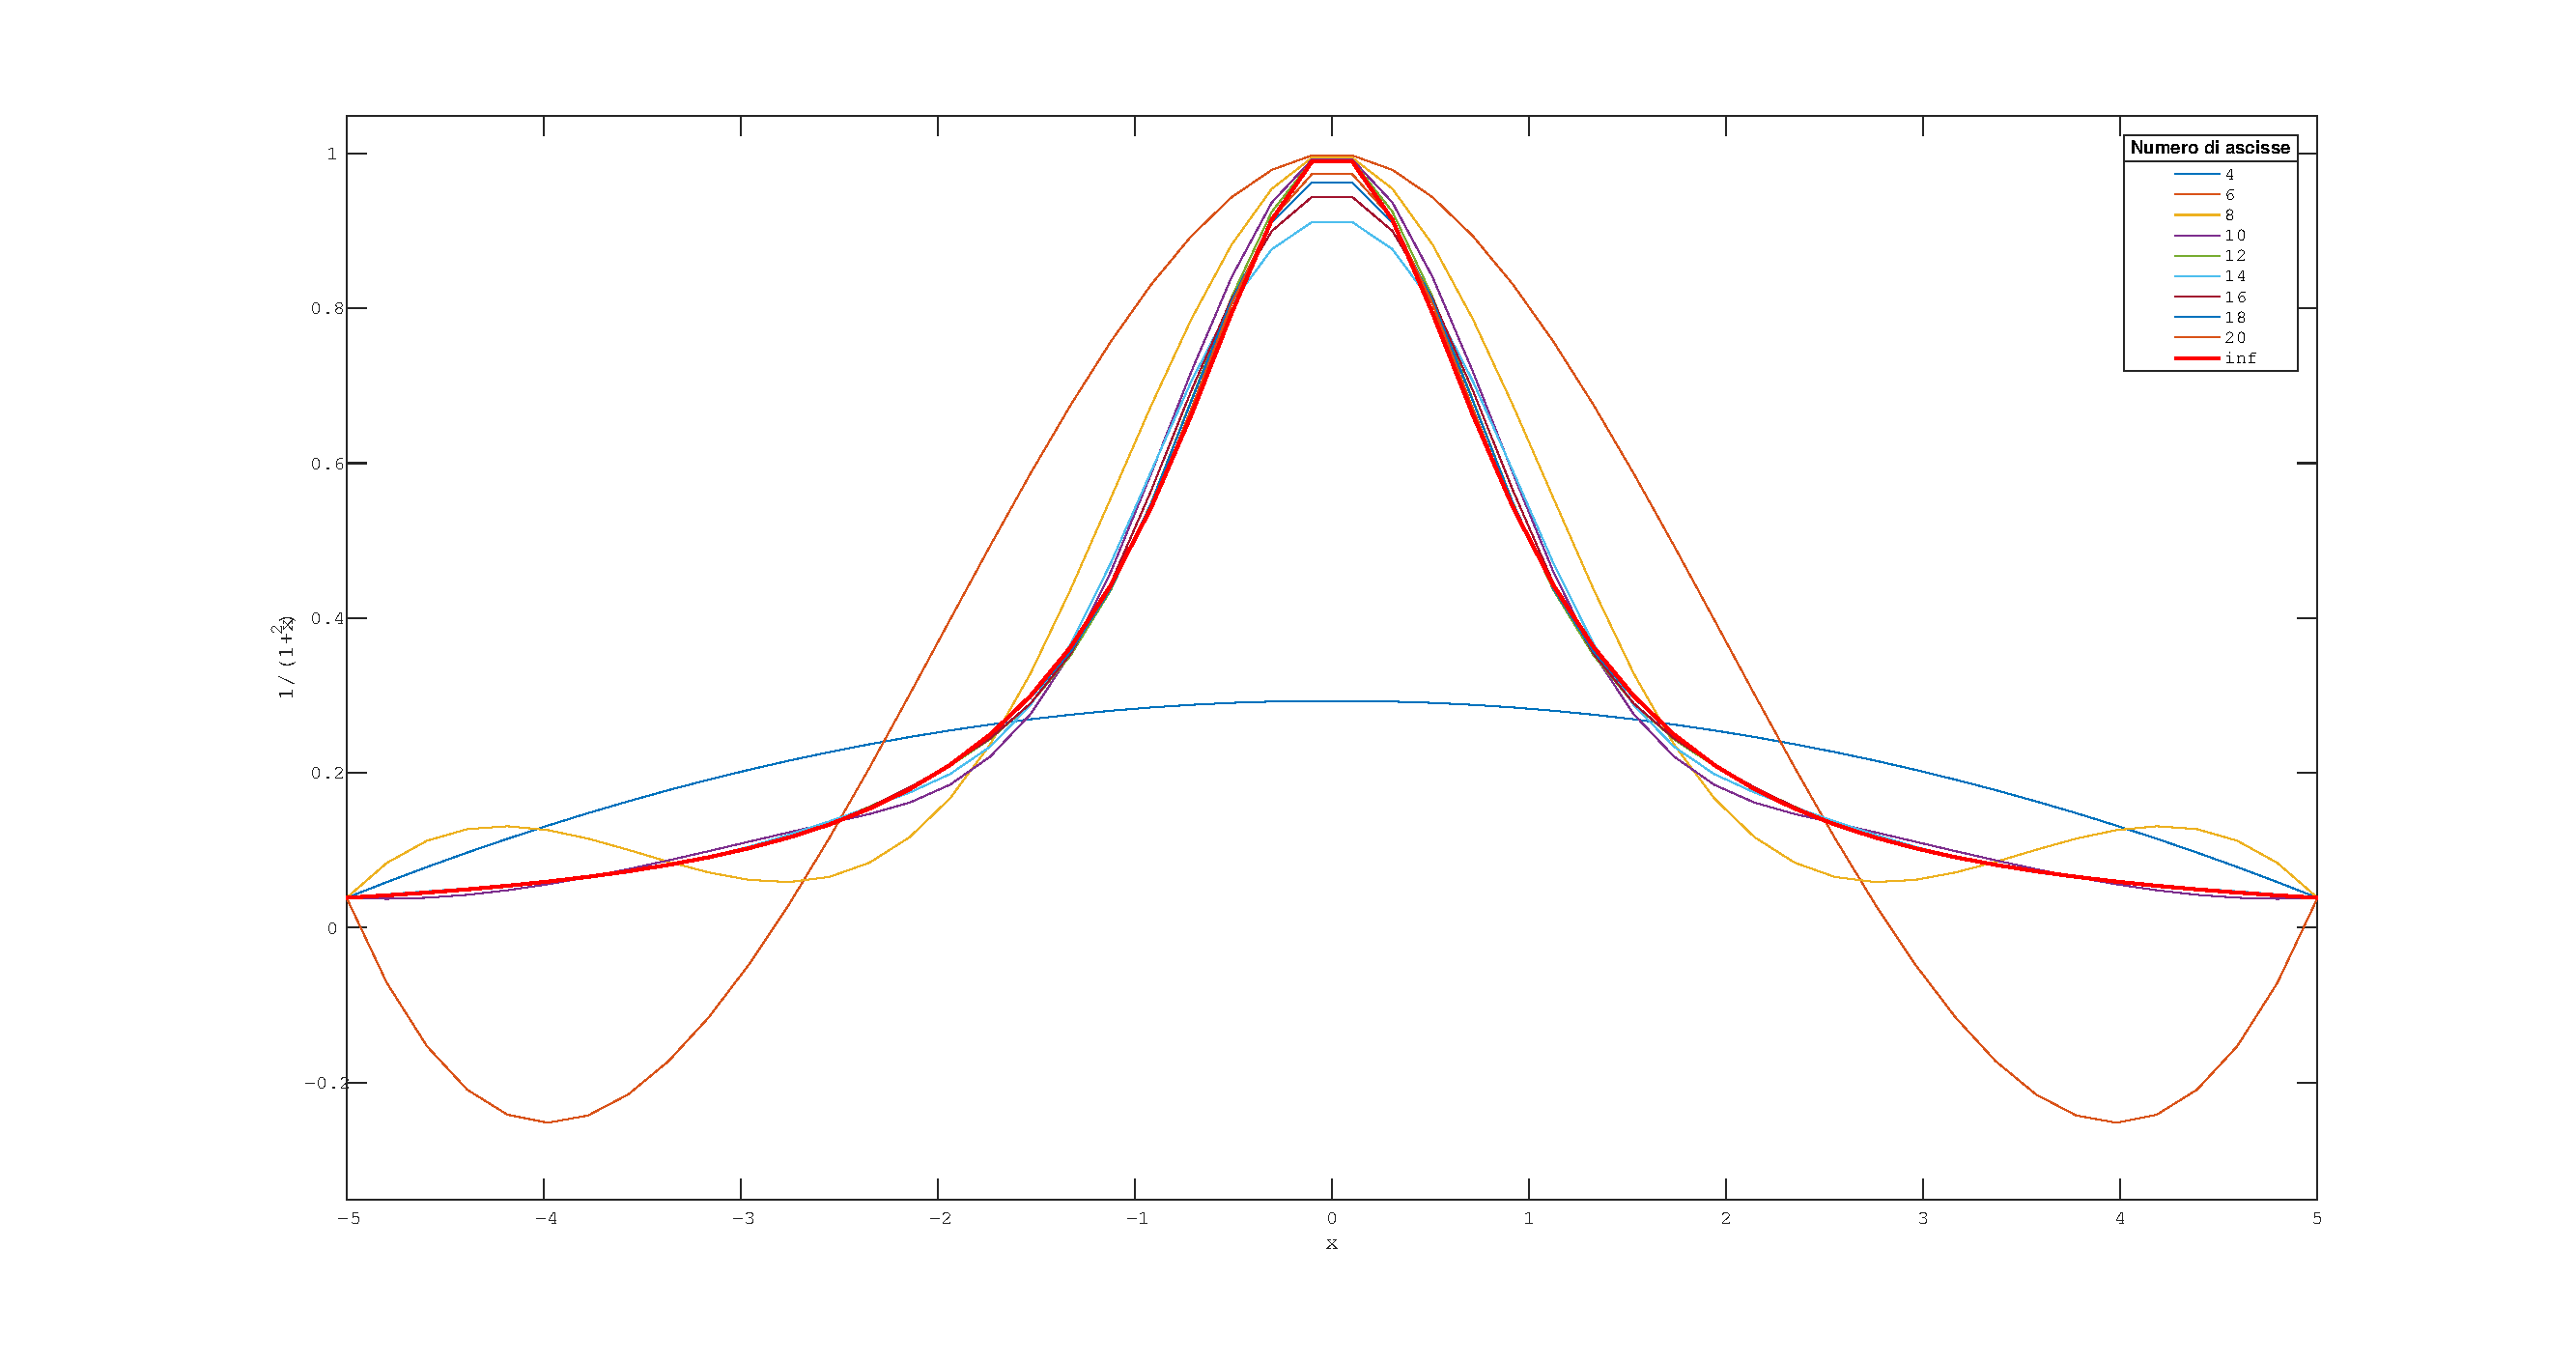
\includegraphics[width=\textwidth]{plot/runge_nak}
\end{figure}
\begin{figure}[h]
\caption{Funzione xsinx not-a-knot}
\label{sin_nak}
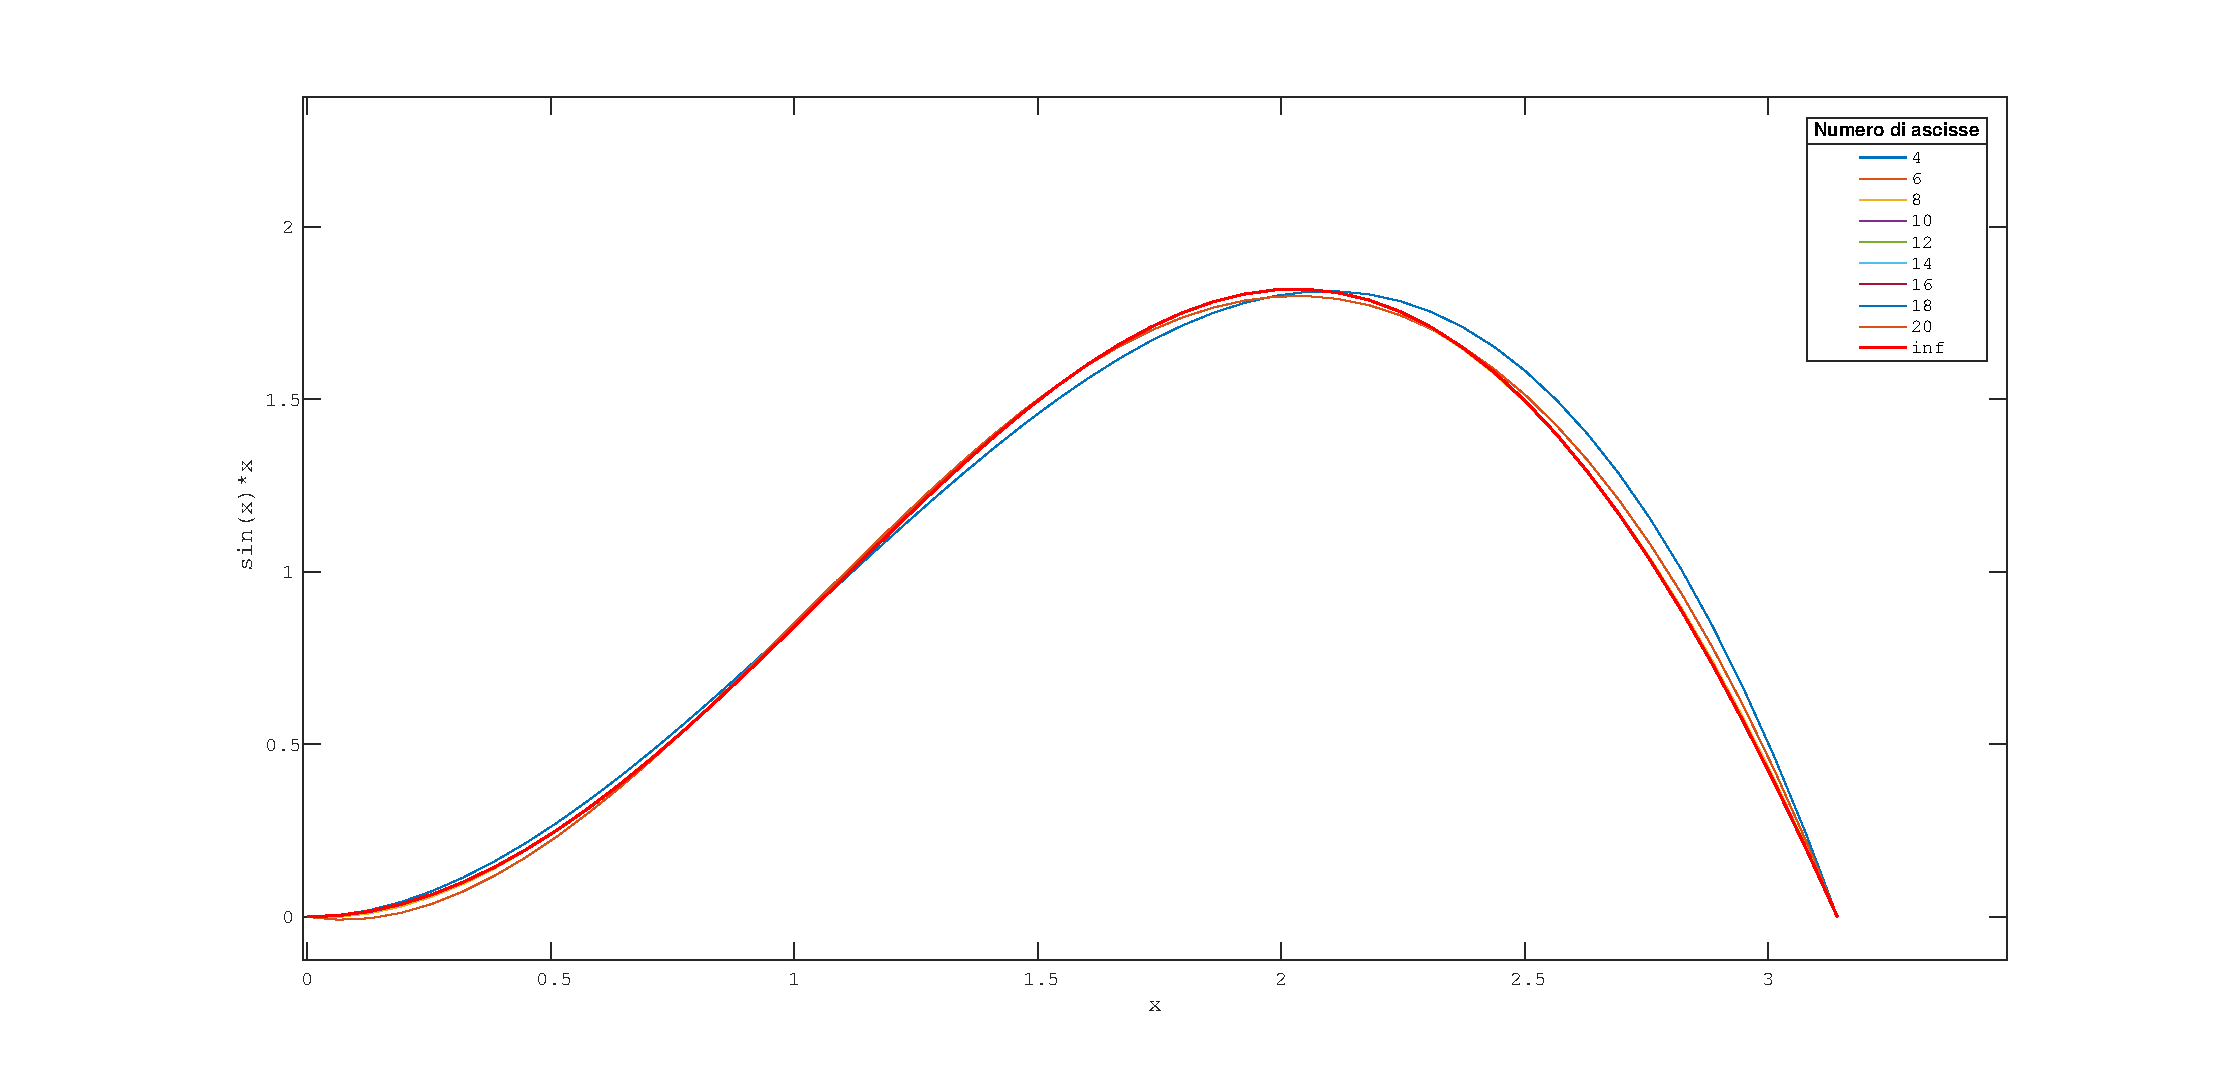
\includegraphics[width=\textwidth]{plot/sin_nak}
\end{figure}
\begin{figure}[h]
\caption{Errori Runge}
\label{erunge_nak}
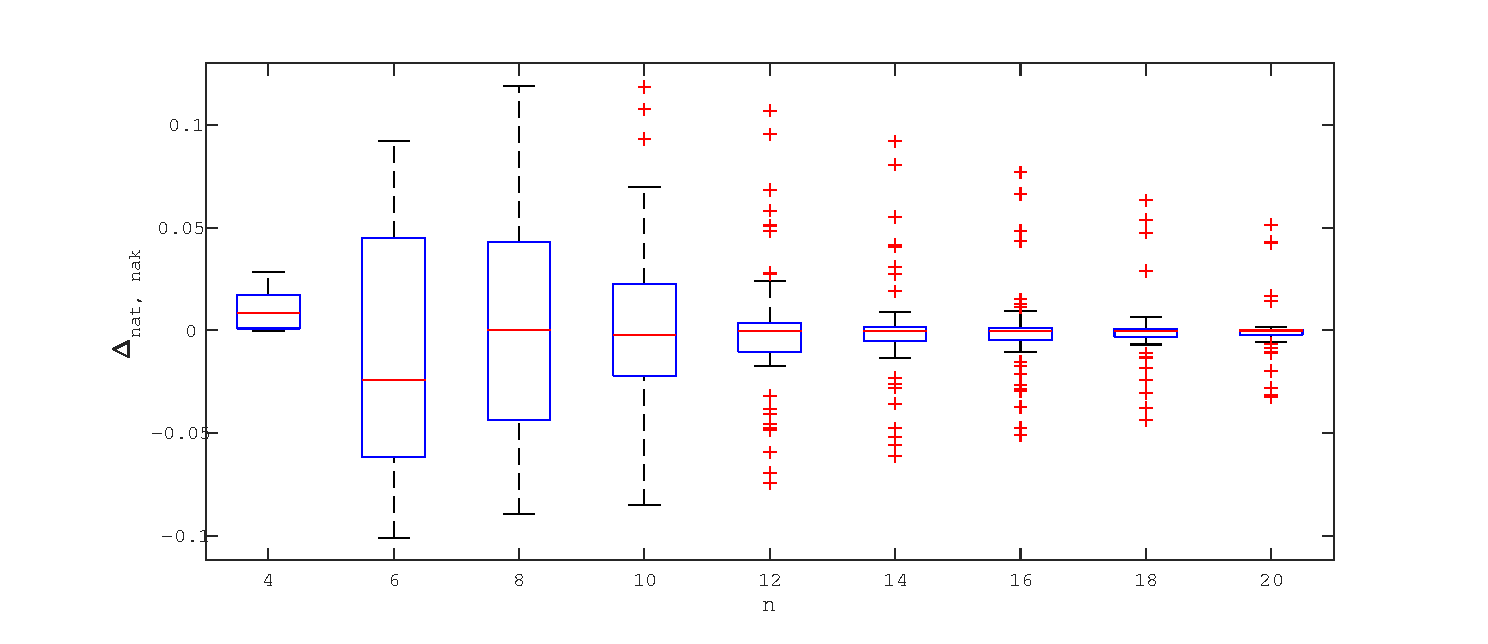
\includegraphics[width=\textwidth]{plot/errors}
\end{figure}
\begin{figure}[h]
\caption{Errori funzione xsinx}
\label{esin_nak}
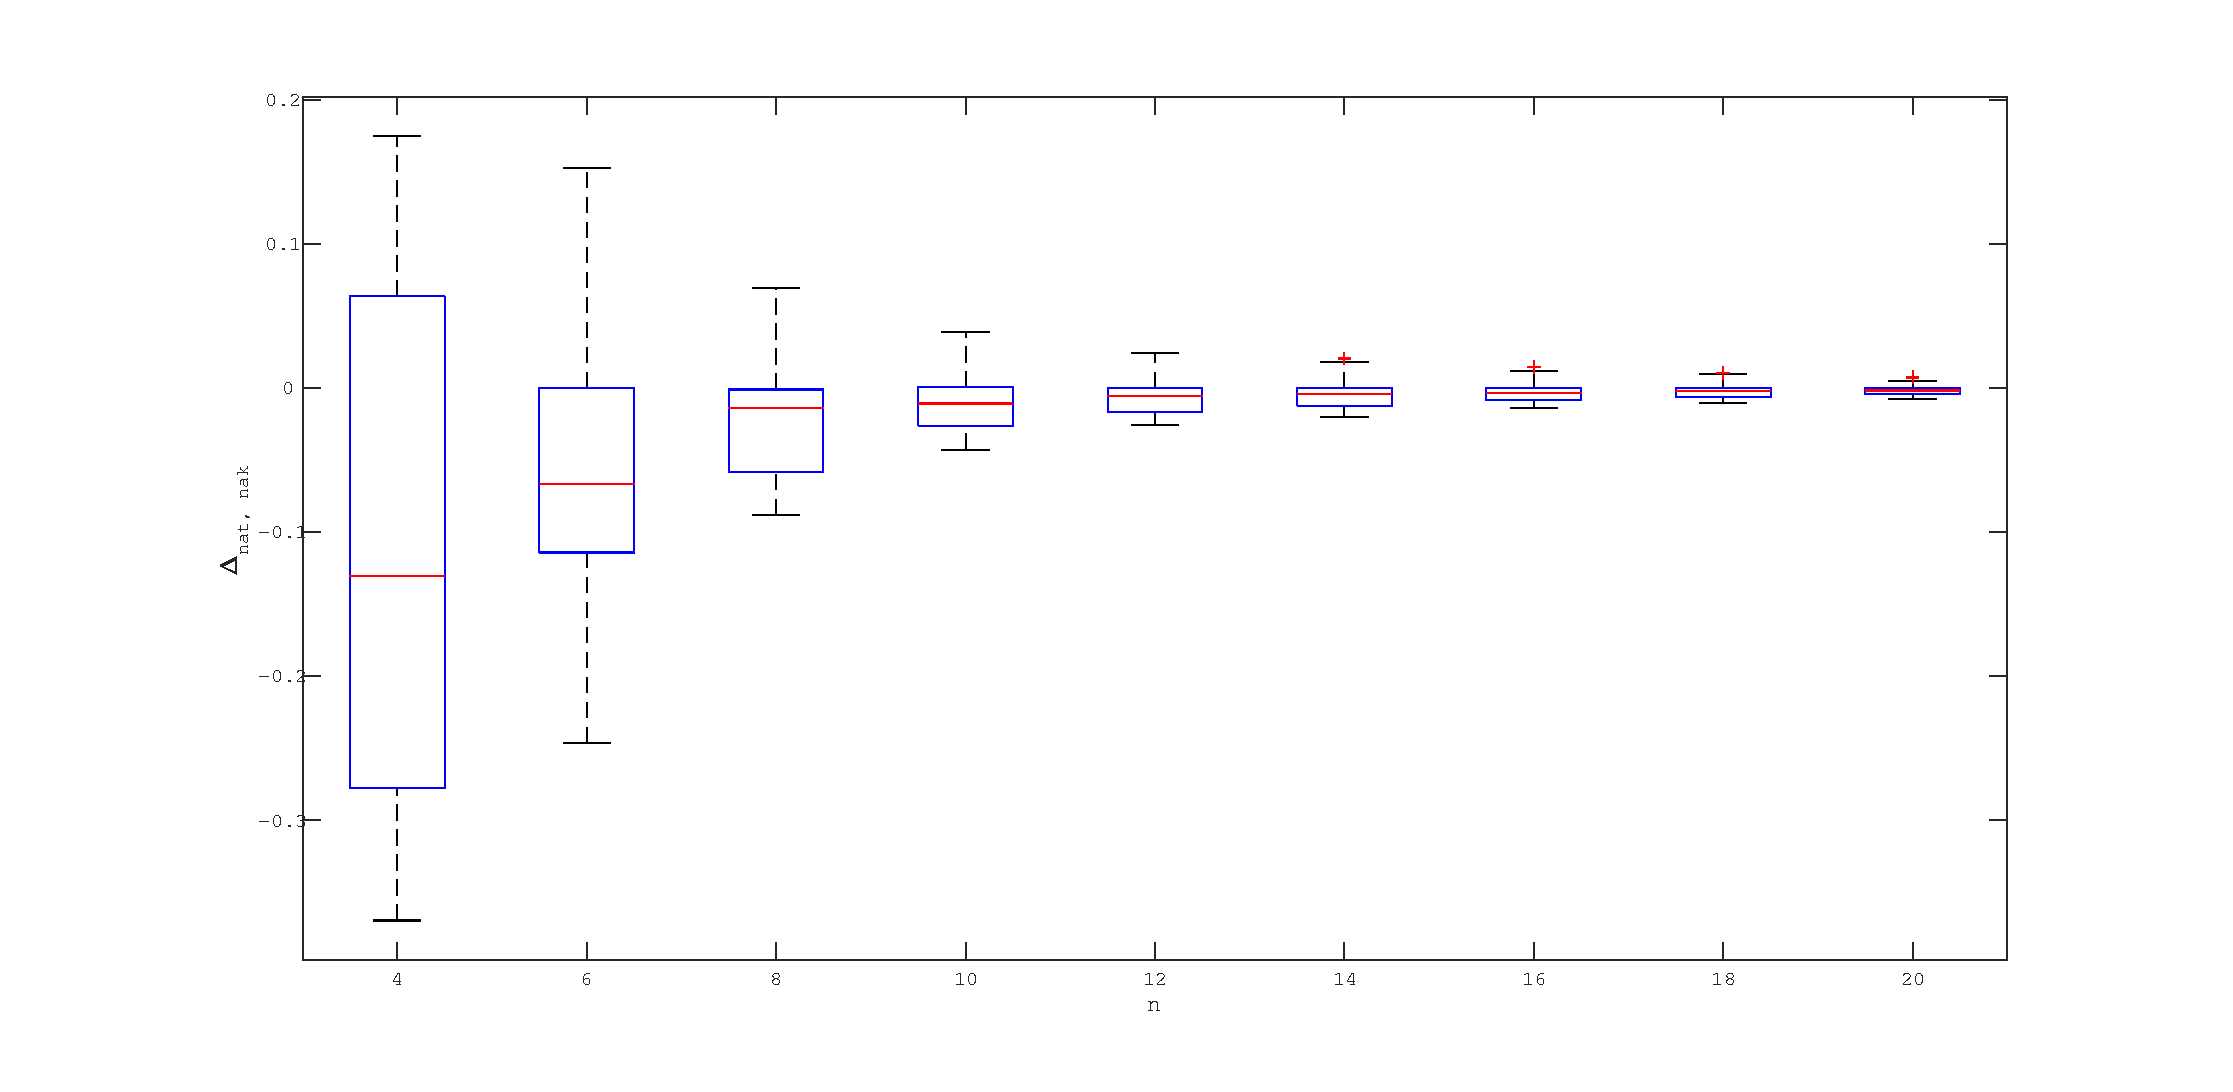
\includegraphics[width=\textwidth]{plot/errors_sin}
\end{figure}
\begin{figure}[h]
\caption{Esercizio 4.10}
\label{fitting}
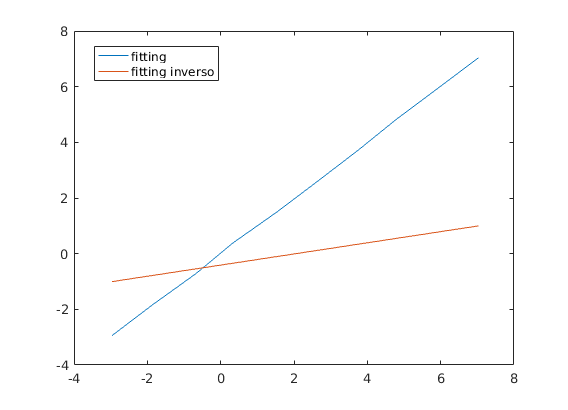
\includegraphics[width=\textwidth]{plot/fittinginv}
\end{figure}
\begin{figure}[h]
\caption{Esercizio 5.2}
\label{PR_comparison}
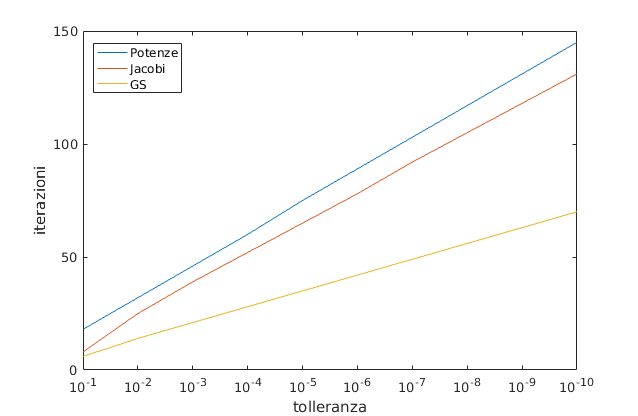
\includegraphics[width=\textwidth]{plot/comparison}
\end{figure}
\begin{figure}[h]
\caption{Esercizio 5.2}
\label{QuadrErr}
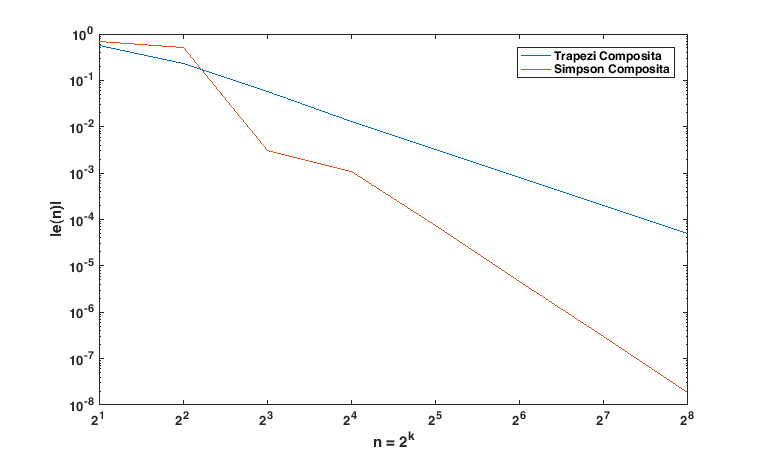
\includegraphics[width=\textwidth]{plot/error}
\end{figure}
\begin{figure}[h]
\caption{Esercizio 5.6}
\label{QuadrRapp}
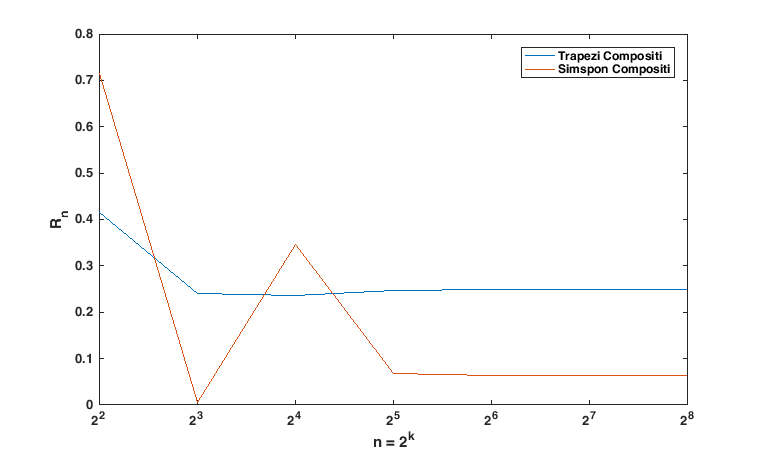
\includegraphics[width=\textwidth]{plot/rapp_err}
\end{figure}

\end{document}
